%
% Libelf by Example
%
% Copyright (c) 2006-2020 Joseph Koshy.  All rights reserved.
%
% Redistribution and use in source and binary forms, with or without
% modification, are permitted provided that the following conditions
% are met:
% 1. Redistributions of source code must retain the above copyright
%    notice, this list of conditions and the following disclaimer.
% 2. Redistributions in binary form must reproduce the above copyright
%    notice, this list of conditions and the following disclaimer in the
%    documentation and/or other materials provided with the distribution.
%
% This software is provided by Joseph Koshy ``as is'' and
% any express or implied warranties, including, but not limited to, the
% implied warranties of merchantability and fitness for a particular purpose
% are disclaimed.  in no event shall Joseph Koshy be liable
% for any direct, indirect, incidental, special, exemplary, or consequential
% damages (including, but not limited to, procurement of substitute goods
% or services; loss of use, data, or profits; or business interruption)
% however caused and on any theory of liability, whether in contract, strict
% liability, or tort (including negligence or otherwise) arising in any way
% out of the use of this software, even if advised of the possibility of
% such damage.
%
% $Id$
%
\documentclass[a4paper,pdftex]{book}

\usepackage{array}
\usepackage{color}
\usepackage{comment}
\usepackage{fancybox}
\usepackage{float}
\usepackage{graphicx}
\usepackage{listings}
\usepackage{makeidx}
\usepackage{tikz}
\usepackage{varioref}
\usepackage{xspace}

\usepackage[colorlinks=true,linkcolor=blue]{hyperref}

% TikZ configuration.
\usetikzlibrary{arrows,calc,chains,mindmap,positioning,shapes.multipart}
\tikzset{every picture/.style={
  >=latex'                      % LaTeX style arrows.
  }
}

% Document-specific LaTeX commands.
\makeatletter
\newcommand{\code}[1]{\texttt{#1}}
\newcommand{\constant}[1]{\texttt{#1}\index{#1@\texttt{#1}}}
\newcommand{\elftoolchainproject}{\href{https://elftoolchain.sourceforge.io/}%
    {ElfToolChain Project}\xspace}%
\newcommand{\function}[1]{\texttt{#1}\index{#1@\texttt{#1}}}%
\newcommand{\filename}[1]{\texttt{#1}}
\newcommand{\firstterm}[1]{\textit{#1}}
\newcommand{\library}[1]{\texttt{#1}}
\newcommand{\parameter}[1]{\texttt{#1}\index{#1@\texttt{#1}}}
\newcommand{\reg}{\textregistered\xspace}
\newcommand{\tableheader}[1]{\small\textbf{#1}}
\newcommand{\tool}[1]{\textbf{#1}}
\newcommand{\trade}{\texttrademark\xspace}
\newcommand{\type}[1]{\texttt{#1}\index{#1@\texttt{#1}}}
\newcommand{\elfdatastructure}[1]{\textsf{#1}}

% Define a new environment "callout" that groups a listing and a
% description list together.  Inside this environment the "\co"
% command may be used to denote a callout location; a corresponding
% "\coref" command may be used at the place in the text that
% references the callout and the two locations will be cross-linked in
% the PDF file generated.
%
% Usage:
%
%   \begin{callout}[color]{UNIQUE-TOKEN}
%    ... \co{M} ...
%    \begin{lstlisting}[escapechar=@]
%       ... @\co{N}@
%    \end{lstlisting}
%    \begin{description}
%    \item[\coref{M}] ... description ...
%    \item[\coref{N}] ... description ...
%    \end{description}
%   \end{callout}
%
% In the typeset text `M' and `N' are made (PDF) targets and rendered
% in a visually distinct way. `UNIQUE-TOKEN' is used to disambiguate
% between different callout environments in the same text.  `color'
% defaults to blue.
\newenvironment{callout}[2][black]{%
  \begingroup\newcommand{\@cocolor}{#1}%
  \setlength{\shadowsize}{1.2pt}%
  \newcommand{\@cogroup}[1]{#2}}{\endgroup}
\newcommand{\@co}[1]{\shadowbox{\color{\@cocolor}#1}}
\newcommand{\co}[1]{%
  \hypertarget{\@cogroup.#1.co}{%
    \hyperlink{\@cogroup.#1.cr}{\@co{#1}}}}
\newcommand{\coref}[1]{%
  \hypertarget{\@cogroup.#1.cr}{%
    \hyperlink{\@cogroup.#1.co}{\@co{#1}}}}

% Add meta-data to the PDF file.
\hypersetup{
  pdftitle={libelf by Example},
  pdfauthor={Joseph Koshy},
  pdfsubject={Handling ELF objects with libelf},
  pdfkeywords={ar archive %
    ELF "ELF sections" %
    GELF %
    loading libelf linker %
    programming %
    "shared library" "shared objects"}
}
\makeatother

\makeindex

\begin{document}
\lstset{language=C,basicstyle=\small\ttfamily,escapechar=@,float}

% Import the title page.
\begin{titlepage}
% A simple title page.
\pagestyle{empty}
\raggedleft

\sffamily
\fontseries{b}

\vspace*{\baselineskip}

\fontsize{60}{64}\selectfont

libelf \\[0.25\baselineskip]
by Example

\vskip 0.55\textheight

\fontsize{32}{36}\selectfont

Joseph Koshy

\end{titlepage}

\setcounter{tocdepth}{1}
\tableofcontents

\chapter*{Preface}

This tutorial introduces the \library{libelf} library being developed
at the \elftoolchainproject on
\href{https://sourceforge.net/}{SourceForge.Net}.  It uses simple
example programs to show how to create ELF processing tools using the
\library{libelf} library. Along the way the tutorial covers the ELF
file format---to the extent needed to understand the example programs
being discussed.

This tutorial would be of interest to software developers who wish to
write software that processes ELF files.

The tutorial's example programs are written using the C programming
language. They should compile out of the box on FreeBSD\trade,
NetBSD\raisebox{0.7ex}{\reg} and other BSD-family operating systems,
and on GNU/Linux\reg with the \filename{libbsd-dev}
package\footnote{\filename{libbsd-dev} is the name of the package in
  Debian and Debian-derived distributions.} (or equivalent) installed.

\section*{Legal Notice}

% Adapted from https://brlcad.org/wiki/BSD_Documentation_License.

Copyright \copyright{} 2006--2020 Joseph Koshy.  All rights reserved.

\vskip.8\baselineskip

Redistribution and use in source (\LaTeX\ format) and ``compiled''
forms (EPUB, HTML, PDF, Postscript, RTF, etc), with or without
modification, are permitted provided that the following conditions are
met:

\begin{itemize}
\item Redistributions of source code (\LaTeX\ format) must retain the
  above copyright notice, this list of conditions and the following
  disclaimer.
\item Redistributions in compiled form (transformed to other
  documentation formats, converted to EPUB, HTML, PDF, Postscript,
  RTF, etc) must reproduce the above copyright notice, this list of
  conditions and the following disclaimer in the documentation and/or
  other materials provided with the distribution.
\item The names of the author and contributors may not be used to
  endorse or promote products derived from this documentation without
  specific prior written permission.
\end{itemize}

THIS DOCUMENTATION IS PROVIDED BY THE AUTHOR AND CON\-TRIBUTORS
``\hskip-0.5ex{}AS~IS'' AND ANY EXPRESS OR IMPLIED WARRANTIES,
INCLUDING, BUT NOT LIMITED TO, THE IMPLIED WARRANTIES OF
MER\-CHANT\-ABILITY AND FITNESS FOR A PARTICULAR PURPOSE ARE
DISCLAIMED.  IN NO EVENT SHALL THE AUTHOR AND CON\-TRIBUTORS BE LIABLE
FOR ANY DIRECT, IN\-DIRECT, INCIDENT\-AL, SPECIAL, EX\-EMPLARY, OR
CON\-SEQUENT\-IAL DAMAGES (INCLUDING, BUT NOT LIMITED TO,
PRO\-CURE\-MENT OF SUBSTITUTE GOODS OR SERVICES; LOSS OF USE, DATA, OR
PROFITS; OR BUSINESS INTERRUPTION) HOWEVER CAUSED AND ON ANY THEORY OF
LIABILITY, WHE\-THER IN CONTRACT, STRICT LIA\-BILITY, OR TORT
(INCLUDING NEGLIGENCE OR OTHER\-WISE) ARISING IN ANY WAY OUT OF THE
USE OF THIS DOCUMENTATION, EVEN IF ADVISED OF THE POSSIBILITY OF SUCH
DAMAGE.

\vskip.8\baselineskip

Many of the designations used by manufacturers and sellers to
distinguish their products are claimed as trademarks. Where those
designations appear in this document, and the author and contributors
were aware of the trademark claim, the designations have been followed
by the ``\raisebox{-.5ex}{\texttrademark}'' or the ``\textregistered'' symbol.

\subsection*{Acknowledgements}

The following people (names in alphabetical order) offered
constructive criticism of this tutorial: Cherry George Mathew, Douglas
Fraser, Hyogeol Lee, Kai Wang, Prashanth Chandra, Ricardo Nabinger
Sanchez, Sam Arun Raj, Wei-Jen Chen and Y.~Giridhar Appaji Nag.  Thank
you, all.

\chapter{Introduction}

ELF \index{ELF} stands for Extensible Linking Format.
It is a file format used by compilers, linkers, loaders and other
tools that manipulate object code.

The ELF specification was released to the public in
1990\index{ELF!history~of} by a group of vendors as an
``\href{https://refspecs.linuxbase.org/elf/elf.pdf}{open
  standard}''. ELF has been widely adopted by industry and by the
open-source community on account of its availability and modern
features.  The ELF standard supports big and little-endian machine
architectures with 32-bit and 64-bit word widths. It supports
cross-compilation, the use of dynamic shared libraries, and the
special compilation needs of the C++ language.\index{ELF!features}

Among the open-source operating systems\index{ELF!in~open-source}, the
RedHat\trade RHL 2.0 Beta release (late summer 1995) and the Slackware
v3.0 (November 1995) release were among the first Linux\reg-based
operating systems to use ELF.  The first ELF based release for
NetBSD\trade was for the DEC Alpha\trade architecture, in release 1.3
(January 1998).  FreeBSD\trade switched to using ELF as its object
format in FreeBSD 3.0 (October 1998).

The \library{libelf} library implements a large set of APIs, known as
the ELF(3) \& GELF(3) APIs.\index{libelf@\texttt{libelf}!API}
These APIs allow you to write software that can run on one kind of
machine architecture, while manipulating ELF objects meant for
another.

There are multiple implementations of the ELF(3)/GELF(3) API set in
the open-source world.  This tutorial is based on the \library{libelf}
library being developed as part of the \elftoolchainproject on
\href{https://sourceforge.net/}{SourceForge.Net}.

The ELF(3)/GELF(3) APIs implemented by the \library{libelf} library
have over 80 callable functions and can be daunting to learn.  This
tutorial offers a gentle introduction to this API set.

\section{On the Structure of This Tutorial}

As you would expect from the tutorial's name, we will be writing
example programs from the very beginning. We will look at a series of
simple but complete programs, each illustrating a different aspect of
the ELF format and the \library{libelf} library's APIs. We will
introduce the necessary ELF related concepts as we go along.

In chapter \vref{chap.getting-started} we cover getting started
with the \library{libelf} library. We look at how to compile and link
an application that uses the library, how to establish a working ELF
version number, how to obtain a handle to a ELF object, and how to
handle any errors reported back by the \library{libelf} library.

In chapter \vref{chap.peering-inside} we study how ELF executables,
relocatable objects and shared objects are laid out. We look at how
the ELF data structure known as the \elfdatastructure{Executable
  Header}\index{executable~header} describes the layout of the rest of
the file.  Along the way we introduce the notions of the ``file
representation''\index{file~representation} and ``memory
representation''\index{memory~representation} of ELF data types, and
look at how the \library{libelf} library enables programs to work
on ELF objects whose word size and endianness differ from their
``native'' size and endianness. We then bring these concepts together
to write a program that displays the contents of the ELF
\elfdatastructure{Executable~Header}\index{executable~header} for an
ELF object.

In chapter \vref{chap.elf-phdr} we study ELF segments. We see how the
segments of a file are described by a \elfdatastructure{Prog\-ram
  Head\-er Table}.\index{program~header~table} We write an example
program to display the program header table entries in an ELF
executable.

In chapter \vref{chap.elf-sections} we look at how data is stored in
ELF sections, and how these sections are described by the ELF
\elfdatastructure{Section Header Table}.\index{section~header~table}
We study how ELF string tables (a special kind of ELF section) are
structured. We then write an example program that traverses an ELF
object, listing the names of its contained sections.

In chapter \vref{chap.creating-elf} we look at how to create new ELF
objects using the \library{libelf} library. We look at how the
\library{libelf} library lays out ELF objects by default, and we look
at how to create ELF objects with custom layouts if the default layout
is not suitable. We look at the correct ordering of individual API
calls when creating ELF objects. Our example program in this chapter
creates a new ELF object from scratch.

We then move on to \tool{ar} archives---in chapter \vref{chap.ar} we
study the structure of these archives. The example program in this
chapter lists the names of files in an \tool{ar} archive.

Finally, we conclude the tutorial with a few suggestions for further
reading.

Figure~\vref{fig.concept.map} offers a graphical overview of the
concepts covered by this tutorial.

\begin{figure}
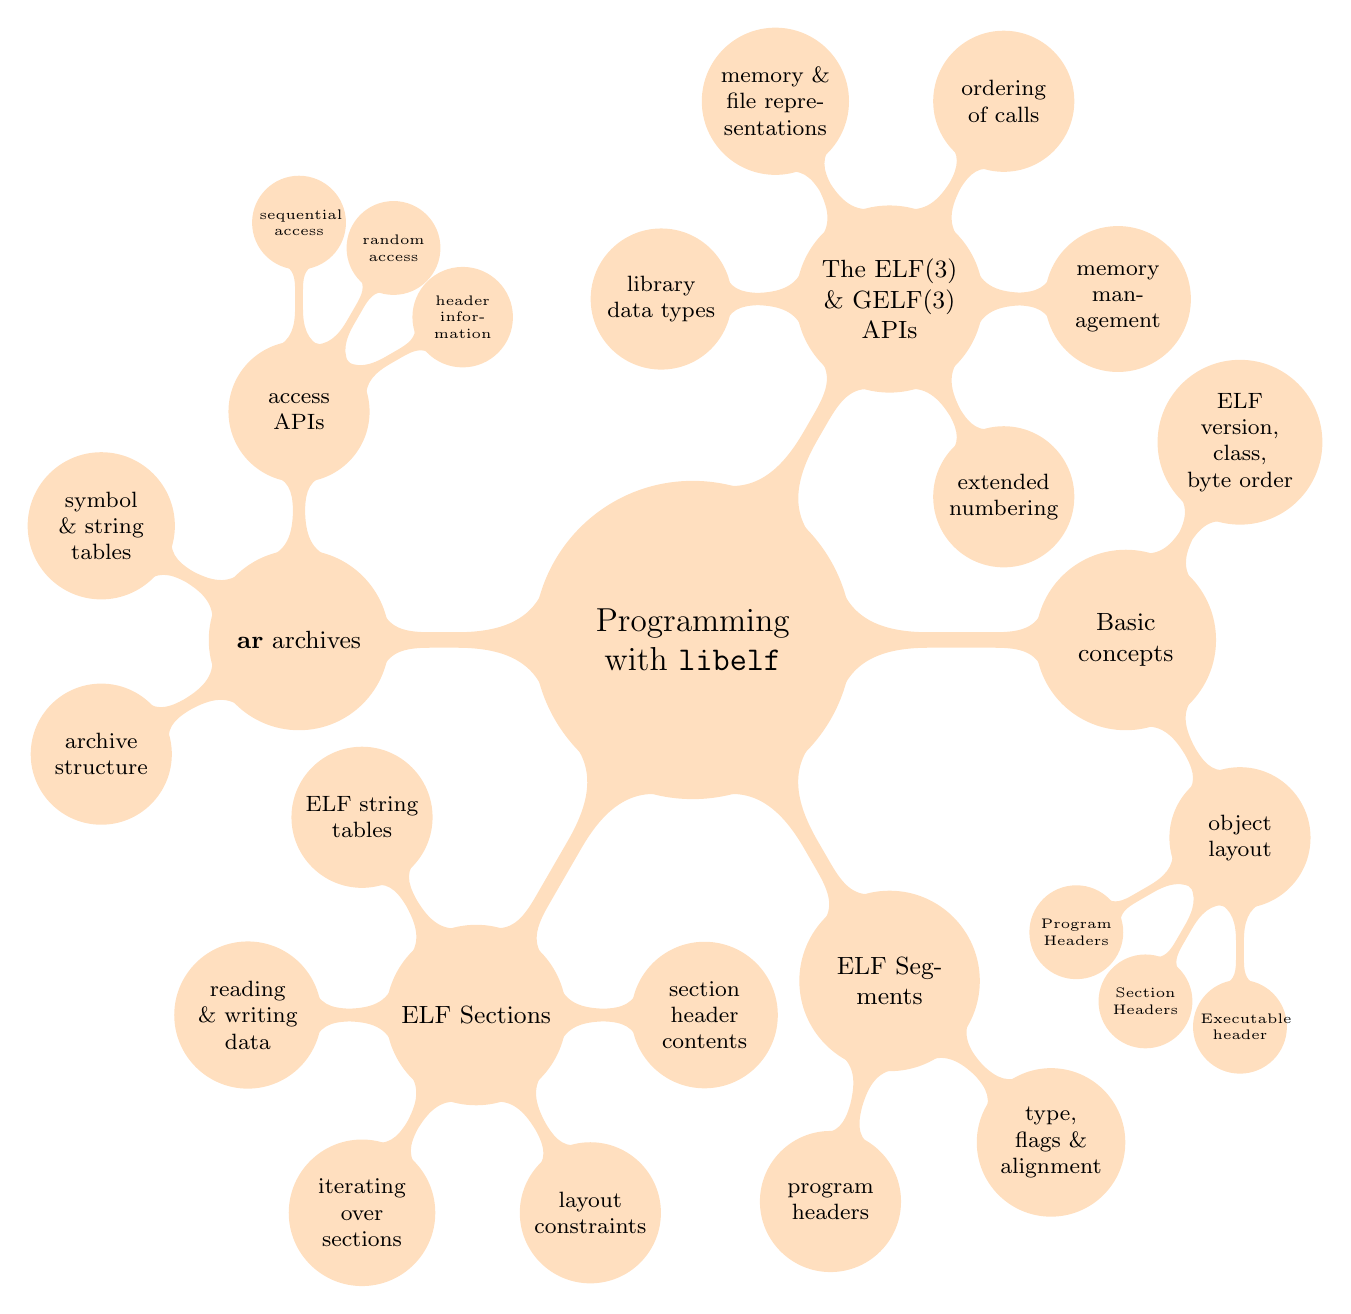
\begin{tikzpicture}[mindmap,concept color=orange!25]
  \node[concept] {Programming with \texttt{libelf}}
    [clockwise from=60]
    child {
      node[concept] {The ELF(3) \& GELF(3) APIs}
      [clockwise from=180]
      child { node[concept] { library data types } }
      child { node[concept] { memory \& file representations } }
      child { node[concept] { ordering of calls } }
      child { node[concept] { memory management } }
      child { node[concept] { extended numbering } }
    }
    child[level distance=5.5cm]  {
      node[concept] {Basic concepts}
      [clockwise from=60]
      child { node[concept] { ELF version, class, byte order } }
      child[grow=-60] {
        node[concept] {object layout}
        [clockwise from=-90]
        child { node[concept] { Executable header } }
        child { node[concept] (shdr) { Section Headers } }
        child { node[concept] (phdr) { Program Headers } }
      }
    }
    child {
      node[concept] (elfseg) {ELF Segments}
      [clockwise from=-45]
      child { node[concept] { type, flags \& alignment } }
      child { node[concept] { program headers } }
    }
    child[level distance=5.5cm] {
      node[concept] (elfsec) {ELF Sections}
      [clockwise from=0]
      child { node[concept] { section header contents } }
      child { node[concept] { layout constraints } }
      child { node[concept] { iterating over sections } }
      child { node[concept] { reading \& writing data } }
      child { node[concept] { ELF string tables } }
    }
    child {
      node[concept] { \tool{ar} archives }
      [clockwise from=-150]
      child { node[concept] { archive structure } }
      child { node[concept] { symbol \& string tables } }
      child { node[concept] { access APIs }
        [clockwise from=90]
        child { node[concept] { sequential access } }
        child { node[concept] { random access } }
        child { node[concept] { header information } }
      }
    };
\end{tikzpicture}
\caption{An overview of the concepts covered in this
  tutorial.}\label{fig.concept.map}
\end{figure}

\chapter{Getting Started}\label{chap.getting-started}

It is time to get a taste of programming with \library{libelf}.

Our first example program (Program 1, listing~\vref{src.prog.1}) will
open the a file named on its command line, and will display the file's
type as recognized by the ELF library.  This example covers the basics
of using \library{libelf}: how to compile a program that uses
\library{libelf}, how to initialize the library, how to handle the
errors reported by the library, and how to release resources cleanly
when done.

\begin{callout}{prog1}
  \lstinputlisting[caption=Program 1, label=src.prog.1]{prog1.txt}

  \begin{description}
  \item[\coref{1}] The functions and dataypes that make up the ELF(3)
    API are declared in the header \filename{libelf.h}.  This file
    must be included by every source file that uses the
    \library{libelf} library.%
    \index{libelf@\texttt{libelf}!header file \filename{elf.h}}

  \item[\coref{2}] The library uses an opaque C type named \type{Elf}
    as a handle to an ELF object.

  \item[\coref{4}] Before the functions in the library can be invoked,
    an application must indicate the version of the ELF specification
    that it expects to use.  This is done by calling the
    \function{elf\_version} function. Calling
    \function{elf\_version} is mandatory---most \library{libelf} APIs
    will return an error if invoked before the expected ELF version is
    set.

    \begin{figure}
      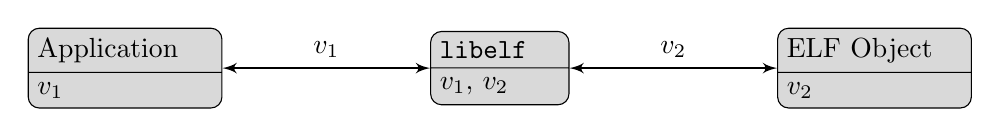
\begin{tikzpicture}[
        version/.style={
          rectangle split,
          rounded corners,
          minimum width=7em,
          text centered,
          fill=black!15,
          draw,
          rectangle split parts=2,
          rectangle split part align={left},
          node distance=7.5em,
        }]
      \node[version] (application) {Application \nodepart{second} $v_1$};
      \node[version,minimum width=5em] (library) [right=of application] { %
       \texttt{libelf} \nodepart{second} $v_1$, $v_2$}
        edge [thick,<->] node[auto,swap] {$v_1$} (application);
      \node[version] (object) [right=of library] { %
        ELF Object \nodepart{second} $v_2$}
        edge [thick,<->] node[auto,swap] {$v_2$} (library);
      \end{tikzpicture}
      \caption{Handling ELF versioning.}\label{fig.versions}
    \end{figure}

    Multiple ELF specification versions could come into play when an
    application reads or writes an ELF object.  In
    figure~\vref{fig.versions} the application program using
    \library{libelf} expects to work with files conforming to version
    $v_1$ of the ELF specification. The ELF object file however
    conforms to ELF specification version $v_2$.  The \library{libelf}
    library understands the semantics of both specification versions
    $v_1$ and $v_2$, and so would be able to (in theory) mediate
    between the application and the ELF object.\index{ELF!versions}

    In practice, the ELF specification's version has not changed since
    its inception; the current version (denoted by the symbol
    \constant{EV\_CURRENT}) is 1.

  \item[\coref{5}] The \function{elf\_begin} function takes an open
    file descriptor and converts it an \type{Elf} handle.

    The second parameter to \function{elf\_begin} can be one of
    `\constant{ELF\_C\_READ}' for opening an ELF object for reading,
    `\constant{ELF\_C\_WRITE}' for creating a new ELF object, or
    `\constant{ELF\_C\_RDWR}' for opening an ELF object for updates.
    The opening mode for the file descriptor \code{fd} should be
    compatible with this parameter: the file descriptor should have
    been opened for reading if used with \constant{ELF\_C\_READ}, for
    writing if used with \constant{ELF\_C\_WRITE} and for updating if
    used with \constant{ELF\_C\_RDWR}.

    The third parameter to \function{elf\_begin} is only used when
    reading \tool{ar} ar\-chives.  We will look at \tool{ar} archive
    processing in chapter~\vref{chap.ar}.

  \item[\coref{6}] When the ELF library encounters an error, it will
    record an error number in an internal location and return a
    sentinel value (e.g., the \code{NULL} value from functions
    that return pointers). The saved error number indicates
    the specific class of error that was encountered. This number can
    be retrieved using the \function{elf\_errno} function.

    Numeric error numbers are not very user-friendly. The
    \function{elf\_errmsg} function returns a human readable string
    describing the error number passed to it.  As a programming
    convenience, an error number of -1 denotes the most recent error
    number that had been saved.

  \item[\coref{3} \coref{7}] The ELF library can operate on \tool{ar}
    archives and ELF objects.  The function \function{elf\_kind}
    returns the kind of object associated with an \type{Elf} handle.
    The return value of the \function{elf\_kind} function is one of
    the values defined by the \type{Elf\_Kind} enumeration in
    \filename{libelf.h}. Currently, the library only recognizes ELF
    files and \tool{ar} archives.

  \item[\coref{8}] When you are done with an \type{Elf} handle you
    should release its resources using the \function{elf\_end}
    function.
  \end{description}
\end{callout}

It is now time to compile and run our first example program.

Save the listing in listing~\vref{src.prog.1} to a file named
\filename{prog1.c}, and then compile and run it as shown in
listing~\vref{scr.prog1}.%
\index{libelf@\texttt{libelf}!linking with}

\begin{callout}{scr1}
  \begin{lstlisting}[basicstyle=\ttfamily, language={},
      caption=Compiling and running prog1,
      label=scr.prog1]
% cc -o prog1 prog1.c -lelf @\co{1}@
% ./prog1 prog1 @\co{2}@
prog1: elf object
% ./prog1 /usr/lib/libc.a @\co{3}@
/usr/lib/libc.a: ar(1) archive
  \end{lstlisting}

  \begin{description}
  \item[\coref{1}] The \code{-lelf} option to the \tool{cc}
    comand informs it to link \tool{prog1} with the \library{libelf}
    library.
  \item[\coref{2}] We then invoke \tool{prog1} on itself. If all went
    well it should recognize its own executable as an ELF object.
  \item[\coref{3}] Here we see that \tool{prog1} recognizes an \tool{ar}
    archive correctly.
  \end{description}
\end{callout}

Congratulations!  You have created your first ELF-aware program using
\library{libelf}.

In the next chapter we will study the ELF format in greater detail.

\chapter{Peering Inside an ELF Object}\label{chap.peering-inside}

In this chapter we will take our first look inside an ELF object. We
will study the ELF data structure known as the ELF
\elfdatastructure{Executable Header} which describes the layout of ELF
objects.  We will look the ``extended numbering'' scheme used by
large ELF objects, and we will study how \library{libelf} makes
it easy to handle non-native ELF objects.

At the end of this chapter we will write a program that prints out
the executable header in an ELF object.

\section{ELF Object Kinds}
ELF supports multiple kinds of objects:

\begin{itemize}
\item \firstterm{Relocatable objects}\index{ELF!relocatable objects}
  contain compiled code along with extra information used by tools
  like linkers. Relocatable objects are usually created by compilers
  when source code is compiled.
\item \firstterm{Executables}\index{ELF!executables} contain
  code in a form that an operating system can directly use to launch a
  process.  The process of forming executables from collections of
  relocatable objects is called
  \firstterm{linking}\index{linking!definition~of}.
\item \firstterm{Dynamically loadable objects}\index{ELF!dynamically
  loadable objects} contain code in a form suitable for
  loading into a running process. Shared
  libraries\index{shared library} are examples of dynamically loadable
  objects.
\item \firstterm{Core files}\index{core files} contain the memory
  image of a process. Core files are usually generated when programs
  crash.
\end{itemize}

Each of these kinds of objects has a different internal structure.

\section{ELF File Layout}

Figure~\vref{fig.elf.layout} shows the layout of a typical ELF
object.\index{ELF!typical layout}

Every ELF object starts with a mandatory data structure known as the
ELF \elfdatastructure{Executable Header}.\index{executable~header}
This header is followed by optional content---depending on the kind of
ELF object, this could be an optional ELF \elfdatastructure{Program
  Header Table}\index{program~header~table} and zero or more ELF
\elfdatastructure{Sections}\index{sections}:

\begin{itemize}
\item The ELF \elfdatastructure{Program Header
  Table}\index{program~header~table} is found in executables and
  dynamically loadable objects.  This data structure contains
  information that is used when the ELF object is loaded into a
  process\index{loading}.  We look at the \elfdatastructure{Program
    Header Table} more closely in chapter~\vref{chap.elf-phdr}.
\item ELF \elfdatastructure{Sections}\index{sections} are present in
  most ELF files. Sections are contiguous regions inside the ELF
  object holding data of a specific kind. ELF sections are described
  by entries in an ELF \elfdatastructure{Section Header
    Table}\index{section~header~table}.
  Chapter~\vref{chap.elf-sections} describes ELF
  \elfdatastructure{Sections} and the ELF \elfdatastructure{Section
    Header Table} in further detail.
\end{itemize}

\begin{figure}
  \begin{center}
  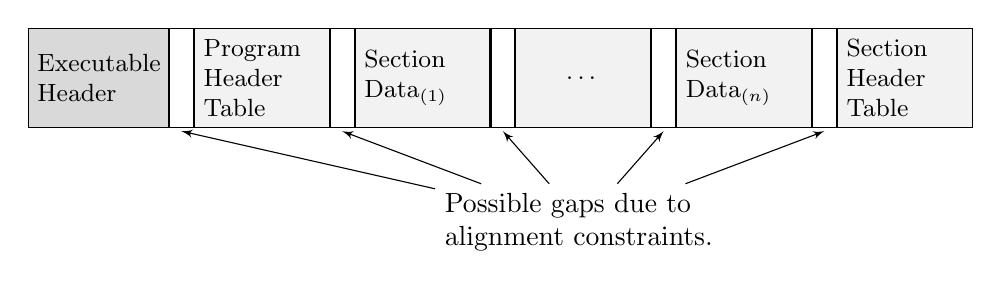
\begin{tikzpicture}[
    start chain,
    node distance=0pt,
    elfpart/.style={
      rectangle,
      draw,
      minimum height=3\baselineskip,
      font=\small,
      text width=4.2em
    },
    gap/.style={
      draw,
      minimum height=3\baselineskip,
      minimum width=2ex
    }]

    % Depict the structure of an ELF object.
    \node[on chain,elfpart,text width=4.4em,fill=black!15] (ehdr)
      {Executable Header};
    \node[on chain,gap]     (g0) {};
    \node[on chain,elfpart,fill=black!5] (phdr) {Program Header Table};
    \node[on chain,gap]     (g1) {};
    \node[on chain,elfpart,fill=black!5]   (s0) {Section Data$_{(1)}$};
    \node[on chain,gap]       (gl0) {};
    \node[on chain,elfpart,text centered,fill=black!5] (sdots) {\ldots};
    \node[on chain,gap]    (gl1) {};
    \node[on chain,elfpart,fill=black!5] (sn) {Section Data$_{(n)}$};
    \node[on chain,gap]       (g3) {};
    \node[on chain,elfpart,fill=black!15,fill=black!5] (shdr)
      {Section Header Table};

    % Label the gaps needed for alignments.
    \node[below=2em of sdots,text width=10em]
      {Possible gaps due to alignment constraints.}
      edge [->] ([yshift=-1pt] g0.south)
      edge [->] ([yshift=-1pt] g1.south)
      edge [->] ([yshift=-1pt] gl0.south)
      edge [->] ([yshift=-1pt] gl1.south)
      edge [->] ([yshift=-1pt] g3.south);
  \end{tikzpicture}
  \end{center}
  \caption{The layout of a typical ELF File.}\label{fig.elf.layout}
\end{figure}


The optional elements of an ELF object are shown with a lighter
background in figure~\vref{fig.elf.layout}.

Let us now take a closer look at the ELF \elfdatastructure{Executable
  Header}.\index{executable~header}

\subsubsection{The ELF Executable Header}\label{sec.ehdr}
Table \vref{src.elf.ehdr} describes the layout of an ELF
\elfdatastructure{Executable Header} using a ``C-like'' notation that
shows the sizes and ordering of its
members.\index{executable~header!layout} In an actual ELF object the
data in the header would be stored using the ELF object's ``native''
byte ordering; this ordering could differ from the byte ordering used
by the program reading the header. 32-bit and 64-bit ELF
\elfdatastructure{Executable Header} structures also have slightly
different layouts due to the differing sizes of their members.

\begin{callout}{ehdr}
  \begin{table}
    \begin{tabular}{rl|l}
      \mbox{} & \tableheader{32 bit Executable Header} &
      \tableheader{64 bit Executable Header} \\ \hline
       & \verb+typedef struct {+&
         \verb+typedef struct {+\\
\co{1} & \verb+  unsigned char e_ident[16];+&
         \verb+  unsigned char e_ident[16];+\\
\co{2} & \verb+  uint16_t      e_type;+&
         \verb+  uint16_t      e_type;+\\
\co{3} & \verb+  uint16_t      e_machine;+&
         \verb+  uint16_t      e_machine;+\\
       & \verb+  uint32_t      e_version;+&
         \verb+  uint32_t      e_version;+\\
       & \verb+  uint32_t      e_entry;+&
         \verb+  uint32_t      e_entry;+\\
\co{4} & \verb+  uint32_t      e_phoff;+&
         \verb+  uint64_t      e_phoff;+\\
\co{5} & \verb+  uint32_t      e_shoff;+&
         \verb+  uint64_t      e_shoff;+\\
       & \verb+  uint32_t      e_flags;+&
         \verb+  uint32_t      e_flags;+\\
       & \verb+  uint16_t      e_ehsize;+&
         \verb+  uint16_t      e_ehsize;+\\
       & \verb+  uint16_t      e_phentsize;+&
         \verb+  uint16_t      e_phentsize;+\\
\co{6} & \verb+  uint16_t      e_phnum;+&
         \verb+  uint16_t      e_phnum;+\\
\co{7} & \verb+  uint16_t      e_shnum;+&
         \verb+  uint16_t      e_shnum;+\\
\co{8} & \verb+  uint16_t      e_shstrndx;+&
         \verb+  uint16_t      e_shstrndx;+\\
       & \verb+} Elf32_Ehdr;+&
         \verb+} Elf64_Ehdr;+\\
    \end{tabular}
    \caption{The ELF \elfdatastructure{Executable Header}.}\label{src.elf.ehdr}
  \end{table}

  \begin{description}
  \item[\coref{1}] Figure \vref{fig.elf.eident} shows the contents of
    the first 16 bytes of the ELF header (the \parameter{e\_ident}
    array).

    \begin{figure}
      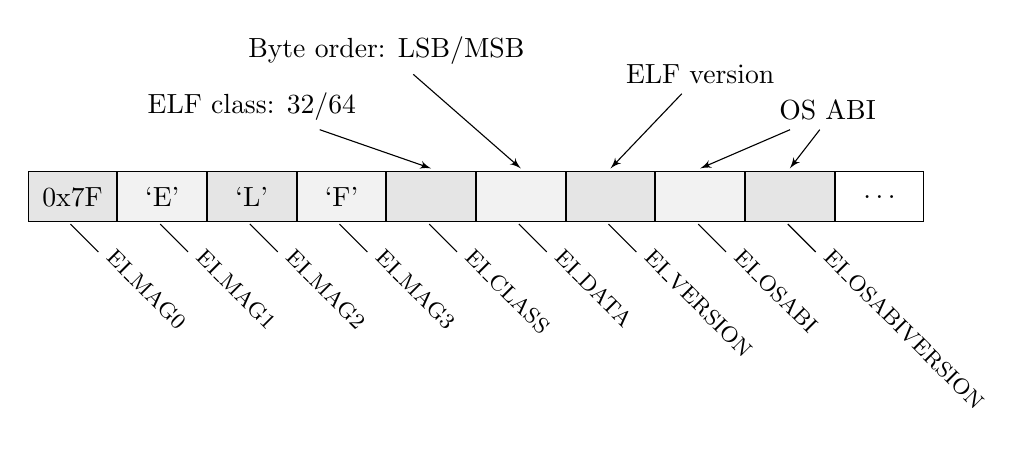
\begin{tikzpicture}[
        start chain,
        node distance=0pt,
        ei/.style={
          on chain,
          draw,
          fill=black!#1,
          minimum width=3.2em,
          minimum height=1.5\baselineskip
        }]

        % Helper macro.
        \def\e#1{\draw[-,rotate=-45]
          ([yshift=-1pt] \tikzchaincurrent.south) -- +(0:0.5cm)
          node[rotate=-45,base right] {\footnotesize EI\_#1}}

        % Draw the e_ident[] array.
        \node[ei=10] (e0) {0x7F};  \e{MAG0};
        \node[ei=5]  (e1) {`E'};   \e{MAG1};
        \node[ei=10] (e2) {`L'};   \e{MAG2};
        \node[ei=5]  (e3) {`F'};   \e{MAG3};
        \node[ei=10] (e4) { };     \e{CLASS};
        \node[ei=5]  (e5) { };     \e{DATA};
        \node[ei=10] (e6) { };     \e{VERSION};
        \node[ei=5]  (e7) { };     \e{OSABI};
        \node[ei=10] (e8) { };     \e{OSABIVERSION};
        \node[ei=0]  (e9) {$\ldots$};

        % Add Labels.
        \node[above=1.5em of e2.north] {ELF class: 32/64}
          edge [->] ([yshift=1pt] e4.north);
        \node[above=3.5em of e3.north east] {Byte order: LSB/MSB}
          edge [->] ([yshift=1pt] e5.north);
        \node[above=2.8em of e7.north] {ELF version}
          edge [->] ([yshift=1pt] e6.north);
        \node[above=1.5em of e8.north east,text width=4em] {OS ABI}
          edge [->] ([yshift=1pt] e7.north)
          edge [->] ([yshift=1pt] e8.north);
      \end{tikzpicture}
      \caption{The layout of the \parameter{e\_ident} array.}%
        \label{fig.elf.eident}
    \end{figure}

    The first 4 bytes of an ELF object always contain 0x7F, 0x45
    (ASCII `E'), 0x4c (ASCII `L') and 0x46 (ASCII `F').

    The next three bytes specify:
    \begin{itemize}
    \item The ELF class\index{ELF!class} of the object---whether it is a 32
      bit ELF object (\constant{ELFCLASS32}) or a 64 bit
      (\constant{ELFCLASS64}) one.
    \item The endianness\index{ELF!endianness} of the object---whether
      little-endian (\constant{ELFDATA2LSB}) or big-endian
      (\constant{ELFDATA2MSB}).
    \item The ELF specification version\index{ELF!version~number}
      number that the object conforms to.  ELF object versioning was
      discussed in chapter~\vref{chap.getting-started}.
    \end{itemize}

    With this information on hand, the \library{libelf} library can
    then interpret the rest of the ELF \elfdatastructure{Executable
      Header} correctly.

  \item[\coref{2}] The \parameter{e\_type} member determines the type
    of the ELF object.  For example, the member would contain the
    value `1' (\constant{ET\_REL}) in a relocatable or the value `3'
    (\constant{ET\_DYN}) in a shared
    object.\index{executable~header!executable type}

  \item[\coref{3}] The \parameter{e\_machine} member describes the
    machine architecture for the ELF object.  Example values are `3'
    (\constant{EM\_386}) for the Intel\reg i386\trade architecture,
    and `20' (\constant{EM\_PPC}) for the 32-bit PowerPC\trade
    architecture.\index{executable~header!executable architecture}

  \begin{figure}
    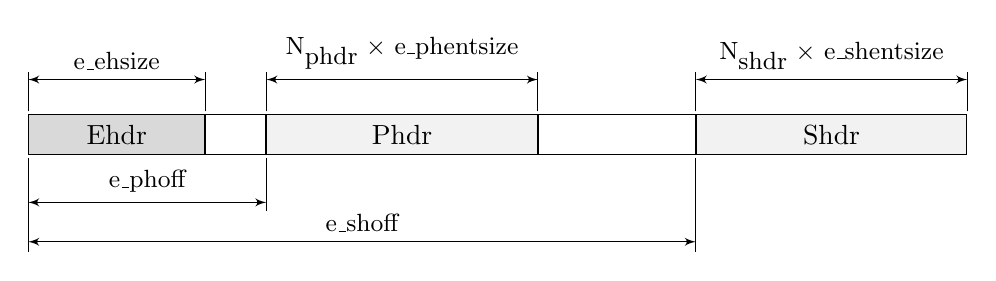
\begin{tikzpicture}[
      start chain,
      node distance=0pt,
      ei/.style={
        on chain,
        draw,
        fill=black!#1,
        minimum height=1.2\baselineskip,
        text centered
      }]

      % Draw the major parts of the ELF object.
      \node[ei=15,text width=2cm] (ehdr) { Ehdr };
      \node[ei=0,text width=1.5em] (gap0) {};
      \node[ei=5,text width=3.2cm] (phdr) { Phdr };
      \node[ei=0,text width=5em] (gap1) {};
      \node[ei=5,text width=3.2cm] (shdr) { Shdr };

      % Draw the marks.
      \def\l#1#2#3{ \draw[-] ([yshift=#2] #1) -- +(90:#3) }; % Helper.

      \l{ehdr.north west}{1pt}{0.5cm};
      \l{ehdr.south west}{-1pt}{-1.2cm};
      \l{ehdr.north east}{1pt}{0.5cm};

      \l{phdr.south west}{-1pt}{-0.67cm};
      \l{phdr.north west}{1pt}{0.5cm};
      \l{phdr.north east}{1pt}{0.5cm};

      \l{shdr.north west}{1pt}{0.5cm};
      \l{shdr.north east}{1pt}{0.5cm};
      \l{shdr.south west}{-1pt}{-1.2cm};

      % Render the labels.
      \def\sz#1#2#3#4{          % Helper macro.
        \draw[<->] ([yshift=#3] #1) -- node [auto] {\small #4 }
          ([yshift=#3] #2)
      }

      \sz{ehdr.north west}{ehdr.north east}{0.44cm}{e\_ehsize};
      \sz{phdr.north west}{phdr.north east}{0.44cm}%
        {N\raisebox{-1ex}{phdr} $\times$ e\_phentsize};
      \sz{shdr.north west}{shdr.north east}{0.44cm}%
        {N\raisebox{-1ex}{shdr} $\times$ e\_shentsize};

      \sz{ehdr.south west}{phdr.south west}{-0.6cm}{e\_phoff};
      \sz{ehdr.south west}{shdr.south west}{-1.1cm}{e\_shoff};

    \end{tikzpicture}
    \caption{The ELF \elfdatastructure{Executable Header} describes
      the layout of the rest of the ELF object.}
    \label{fig.elf.ehdr-layout}
  \end{figure}

  \item[\coref{4} \coref{5}] The ELF \elfdatastructure{Executable
    Header} also describes where to find the ELF
    \elfdatastructure{Program Header Table} and the
    \elfdatastructure{Section Header Table}, if these data structures
    are present in the ELF object (Figure~\vref{fig.elf.ehdr-layout}).

    The \parameter{e\_phoff} and \parameter{e\_shoff} members contain
    the file offsets at which the ELF \elfdatastructure{Program Header
      Table} and the ELF \elfdatastructure{Section Header Table}
    reside in the ELF object.  These members are zero if the file does
    not contain the corresponding data structures.  The sizes of these
    tables are determined by the \parameter{e\_phentsize} and
    \parameter{e\_shentsize} members of the executable header, in
    conjunction with the number of entries in these tables.%
    \index{section~header~table!layout in file}%
    \index{section~header~table!entry size}%
    \index{program~header~table!layout}%
    \index{program~header~table!entry~size}

    The ELF \elfdatastructure{Executable Header} describes its own
    size (in bytes) in member
    \parameter{e\_ehsize}.\index{executable~header!own size}

  \item[\coref{6} \coref{7}] The \parameter{e\_phnum} and
    \parameter{e\_shnum} members contain the number of ELF program
    header table entries and section header table entries
    respectively.

    These fields are only 2 bytes wide, so if an ELF object has a
    large number of sections or program header table entries, then a
    scheme known as ``Extended Numbering''\index{extended~numbering}
    (section~\vref{sec.extended-numbering}) is used to encode the
    actual number of sections or program header table entries.  When
    extended numbering is in use these fields will contain special
    values instead of actual counts.

  \item[\coref{8}] When an ELF object contains sections, the names of
    these sections are stored in a separate string table section.  We
    will cover ELF string tables in more detail in
    section~\vref{sec.shdr.strtab}.\index{sections!names!string~table}

    The \parameter{e\_shstrndx} member stores the section index of
    this string table (possibly using ``Extended Numbering'', see
    section \vref{sec.extended-numbering}). This allows tools
    processing the ELF object to use the correct string table for
    looking up section names.
  \end{description}

  The \parameter{e\_entry} and \parameter{e\_flags} members are used
  for executables. These members are placed in the executable header
  for easy access at program load time.  We will not look at these
  further in this tutorial.\index{executable~header!program entry
    point}\index{executable~header!flags}
\end{callout}

\section{Extended Numbering}\label{sec.extended-numbering}%
\index{extended~numbering}

The \parameter{e\_shnum}, \parameter{e\_phnum} and
\parameter{e\_shstrndx} members of the ELF
\elfdatastructure{Executable Header} are 2 bytes long and are not wide
enough to represent numbers larger than 65535. We therefore need a
different way of encoding these numbers for ELF objects with a large
number of sections or segments.\index{extended~numbering!need for}

When extended numbering is in use, the actual values of these members
will be stored in the normally unused zeroth section header table
entry.\footnote{Section header table entries are covered in more
  detail in section~\vref{chap.elf-sections}.}

\begin{itemize}
\item The true number of sections will stored in the
  \parameter{sh\_size} field of the zeroth section header table entry,
  while the \parameter{e\_shnum} member of the ELF executable header
  will be set to zero.
\item The actual number of program header table entries will be stored
  in the \parameter{sh\_info} field of the zeroth section header table
  entry, while the \parameter{e\_phnum} member of the executable
  header will be set to the value \constant{PN\_XNUM}
  (0xFFFF).\index{extended~numbering!program headers}
\item The true index of the section name string table will be stored
  in the \parameter{sh\_link} field of the zeroth entry of the section
  header table, while the \parameter{e\_shstrndx} member of the
  executable header will be set to the value \constant{SHN\_XINDEX}
  (0xFFFF).\index{extended~numbering!sections}
\end{itemize}

What all this means is that you should use the functions
\function{elf\_getphdrnum}, \function{elf\_getshdrnum} and
\function{elf\_getshdrstrndx} to read the value of these members from
an \type{Elf} descriptor. Directly using the values of the
\parameter{e\_phnum}, \parameter{e\_shnum} and \parameter{e\_shstrndx}
members of the executable header is likely to be wrong.

\section{The ELf32, Elf64 and GElf APIs}

The ELF(3) API is defined in terms of ELF class-dep\-endent types
(\type{Elf32\_Ehdr}, \type{Elf64\_Shdr}, etc). Consequently many
operations on ELF handles in the ELF(3) API have both 32- and 64- bit
variants.

For example, in order to retrieve an ELF executable header from a 32
bit ELF object we would use the function \function{elf32\_getehdr},
which would return a pointer to an \type{Elf32\_Ehdr} structure.  For
a 64-bit ELF object, we would need to use \function{elf64\_getehdr},
which would return a pointer to an \type{Elf64\_Ehdr} structure.

This duplication is awkward when you want to write applications that
need to process either class of ELF objects.%
\index{ELF!class~agnostic~APIs}.

The GELF(3)\index{GELF API} APIs instead provide a way to write
applications that can handle objects of both ELF classes without code
duplication.  These APIs are defined in terms of ``generic'' C types
that are large enough to hold their corresponding 32-bit and 64- bit
ELF types. The GELF(3) data types have names that start with
\code{GElf\_}, and the functions have names that start with
\code{gelf\_}.  You can freely mix calls to GELF(3) and ELF(3)
functions in your code.

The downside to using the GELF(3) APIs is the small cost of the
copying and conversion that happens behind the scenes inside
\library{libelf}.\index{GELF API!downsides to} This overhead is
usually insignificant for most programs.

\section{File and Memory Representations}\label{sec.representations}

\begin{figure}
  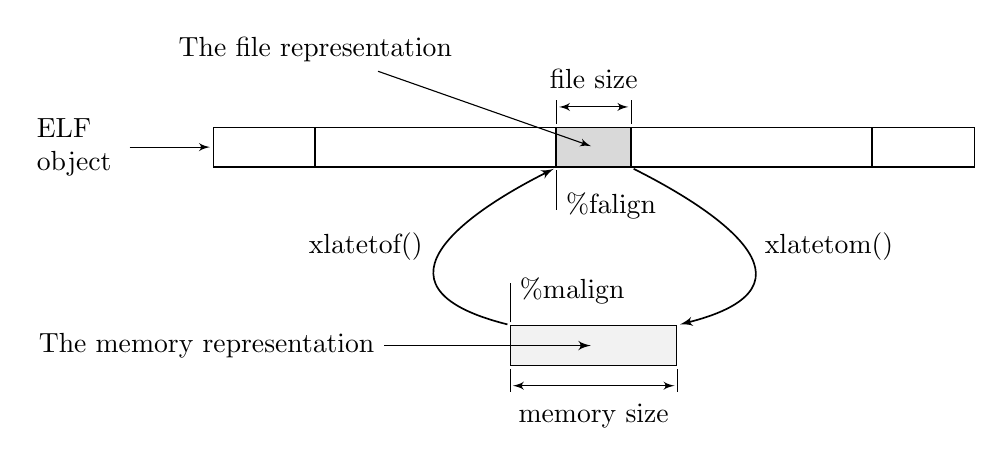
\begin{tikzpicture}[
    start chain,
    node distance=0pt,
    ef/.style={
      on chain,
      draw,
      minimum height=1.2\baselineskip,
      text centered
    }]

    % Helper macros.
    \def\l#1#2#3{ \draw[-] ([yshift=#2] #1) -- +(90:#3) }
    \def\sz#1#2#3#4{
        \draw[<->] ([yshift=#3] #1) -- node [auto] {\small #4 }
          ([yshift=#3] #2)
      }

    % Draw a skeletal ELF object.
    \node[ef,text width=3em] (ehdr) {};
    \node[ef,text width=8em] (g0) {};
    \node[ef,text width=2em,fill=black!15] (file) {};
    \node[ef,text width=8em] (g1) {};
    \node[ef,text width=3em] (shdr) {};

    % Label the ELF object as a whole.
    \node[left=3em of ehdr.west,text width=3em] { ELF object }
      edge [->,shorten >=1pt] (ehdr.west);

    % Label the box denoting the file representation of data.
    \node[above=2em of ehdr.north east] {The file representation}
      edge [->,shorten >=1pt] (file.center);

    % Place tick marks around the file representation box.
    \l{file.north west}{1pt}{0.3cm};
    \l{file.north east}{1pt}{0.3cm};
    \l{file.south west}{-1pt}{-0.5cm};

    % Show the size of the file representation and its alignment.
    \draw[<->,shorten >=1pt,shorten <=1pt]
      ([yshift=0.25cm] file.north west) --
      node [above=0.75ex,text centered,text width=5em] {file size}
      ([yshift=0.25cm] file.north east);
    \node[below right=0.2cm and 0cm of file.south west] {\%falign};

    % Draw and label the memory representation of the data.
    \node[below=2cm of file.south,minimum width=6em,
       minimum height=1.2\baselineskip,draw,fill=black!5]
      (mem) { };
    \node[left=1.6cm of mem]
      {The memory representation}
      edge [->,semithick,shorten >=1pt] (mem.center);

    % Show the memory alignment.
    \l{mem.north west}{1pt}{0.5cm};
    \node[above right=0.15cm and 0cm of mem.north west] {\%malign};

    % Indicate the memory size.
    \l{mem.south west}{-1pt}{-0.3cm};
    \l{mem.south east}{-1pt}{-0.3cm};
    \draw[<->,shorten >=1pt,shorten <=1pt]
      ([yshift=-0.25cm] mem.south west) --
      node [below=0.75ex] {memory size}
      ([yshift=-0.25cm] mem.south east);

    % Draw the arrows denoting translation between file and memory.
    \draw[->,semithick,shorten >=1pt,shorten <=1pt] (file.south east) ..
      controls ++(1,-.5) and ++(2,0.5) ..
      (mem.north east) node[midway,right=1ex] {xlatetom()} ;
    \draw[<-,semithick,shorten >=1pt,shorten <=1pt] (file.south west) ..
      controls ++(-1,-.5) and ++(-2,0.5) ..
      (mem.north west) node[midway,left=1ex] {xlatetof()} ;
  \end{tikzpicture}
  \caption{The relationship between the file and memory representation
    of an ELF data structure.}\label{fig.representations}
\end{figure}

ELF objects use the native word width, enddianness and data alignment
rules of the machine they are intended for.  These could be different
from the native word width, enddianness and data alignment rules for
the machine that the program reading the ELF object is running on.

ELF data structures therefore have two distinct
representations:\index{object~representation}

\begin{itemize}
\item An \emph{in-memory representation} that obeys the constraints
  for the machine architecture that the program handling the ELF
  object is running on.
\item An \emph{in-file representation} that corresponds to the target
  architecture for the ELF object.
\end{itemize}

Figure \vref{fig.representations} depicts the relationship between the
in-file and in-memory representations of an ELF data structure.  This
figure shows that:\index{object~representation!file vs memory}

\begin{itemize}
\item The size of an ELF data structure in the file could be different
  from its size in memory.
\item The alignment restrictions placed on the data structure (denoted
  by \code{\%falign} and \code{\%malign} in the figure)
  could differ.
\item The byte ordering of data in the file could be different
  from that in memory.
\end{itemize}

When using \library{libelf} you do not need to handle these
differences in your code---\library{libelf} will handle the
conversions of in-memory ELF data structures to and from their in-file
representations automatically.  For example, when we read in the ELF
executable header in program~\vref{src.prog.2} below, the
\library{libelf} library will automatically do the necessary
byteswapping and alignment adjustments for us.%
\index{ELF!class~agnostic~APIs}%
\index{libelf@\texttt{libelf}!automatic~data~conversion}

If you need finer-grain control over the conversion process, you could
use the \code{elf\textit{NN}\_xlatetof} and
\code{elf\textit{NN}\_xlatetom} functions offered by \library{libelf}.
\index{libelf@\texttt{libelf}!manual~data~conversion} We don't look at
these functions in this introductory tutorial.

\section{Example: Reading an ELF Executable Header}

Let us create a program that will print out the ELF
\elfdatastructure{Executable Header} present in an ELF object. Our
example program will use the GELF(3) API set.\index{GELF API}

\begin{callout}{prog2}
  \lstinputlisting[caption=Program 2, label=src.prog.2]{prog2.txt}

  \begin{description}
  \item[\coref{1}] Source code that uses the GELF(3) APIs should
    include \filename{gelf.h} header file.%
    \index{libelf@\texttt{libelf}!header file \filename{gelf.h}}

  \item[\coref{2}] The GELF(3) functions always operate on a local
    copies of data structures.  The \type{GElf\_Ehdr} type has fields
    that are large enough to contain values for a 64 bit ELF
    executable header.

  \item[\coref{3}] We use the \function{elf\_begin} function to obtain
    an \type{Elf} handle opened for reading.

  \item[\coref{4}] We retrieve the ELF executable header using
    function \function{gelf\_getehdr}.  This function will translate
    the ELF executable header in the ELF object to its corresponding
    in-memory representation in the C type \type{GElf\_Ehdr}.  For
    example, if a 32-bit ELF object is being examined, then the values
    in its executable header would be appropriately
    expanded and/or byte swapped by this function.%
    \index{executable~header!retrieval of}

  \item[\coref{5}] The \function{gelf\_getclass} function retrieves
    the ELF class of the object being examined.%
    \index{ELF!class!retrieval of}

  \item[\coref{6}] We use the \function{elf\_getident} function to
    retrieve the contents of the \parameter{e\_ident} array from the
    ELF descriptor.  These bytes would also be present in the
    \parameter{e\_ident} member of the \elfdatastructure{Executable
      Header} structure. We print the
    first few bytes of the \parameter{e\_ident} byte array.

  \item[\coref{7}] After printing out the values of the bytes in the
    \parameter{e\_ident} array, we print the values of some of the
    fields of the ELF executable header structure.

  \item[\coref{8}] We use the function \function{elf\_getphdrnum}, to
    retrieve the count of program header table entries in the ELF
    object.

  \item[\coref{9}] We use the \function{elf\_getshdrnum} function to
    retrieve the number of sections in the ELF object.

  \item[\coref{10}] We use the function \function{elf\_getshdrstrndx}
    function to retrieve the index of the section name string table in
    the object.
  \end{description}
\end{callout}

Save the program in listing~\vref{src.prog.2} to a file named
\filename{prog2.c}, and compile and run it as shown in
listing~\vref{scr.prog2}.%
\index{libelf@\texttt{libelf}!linking with}

\begin{callout}{scr2}
  \newcommand{\at}{@}
  \begin{lstlisting}[language={}, basicstyle=\small\ttfamily,
      label=scr.prog2, caption=Compiling and Running prog2]
% cc -o prog2 prog2.c -lelf @\co{1}@
% ./prog2 prog2 @\co{2}@
prog2: 64-bit ELF object
    e_ident[0..8]    ['\^?' 7F] ['E' 45] ['L' 4C] ['F' 46] \
    ['\^B' 2] ['\^A' 1] ['\^A' 1] ['\^I' 9] ['\^@\at@' 0]
    e_type           0x2
    e_machine        0x3e
    e_version        0x1
    e_entry          0x400a10
    e_phoff          0x40
    e_shoff          0x16f8
    e_flags          0x0
    e_ehsize         0x40
    e_phentsize      0x38
    e_shentsize      0x40
    (shnum)          0x18
    (shstrndx)       0x15
    (phnum)          0x5
  \end{lstlisting}
  \begin{description}
  \item[\coref{1}] The process for compiling and linking a GELF(3)
    application is the same as for other \library{libelf} based
    programs.

  \item[\coref{2}] We run our program on itself.  This listing in this
    tutorial was generated on an AMD64\trade machine running FreeBSD\trade.
  \end{description}

  You should now run \tool{prog2} on other object files that you have
  lying around.  Try it on a few non-native ELF object files too.
\end{callout}

\chapter{Examining the Program Header Table}\label{chap.elf-phdr}

Before a program on disk can be executed by a processor it needs to
brought into system memory. The technical name for this process is
``loading''.\index{loading}

When loading an ELF program into memory, the operating system views it
as comprising of distinct parts, where each part has a particular
characteristic. For example, one part of the program could contain
read-only data that needs to be loaded at a specific virtual memory
address. Another part could contain executable code.\index{segments}
Each such part of the ELF object is called an ELF
\elfdatastructure{Segment}\index{segments!definition~of}.

By way of an example, the FreeBSD\trade operating system expects
programs to contain a segment containing executable
code.\index{segments!example~layout} This segment is called the
program's ``\filename{text}'' segment. A \filename{text} segment would
usually be loaded into memory with `read' and `execute' permissions.
Multiple processes using the same executable could potentially share
the same \filename{text} segment.  FreeBSD programs would usually have
\filename{data} segments too; these segments are placed in memory with
`read' and `write' permissions, and made private to each process.

Like executables, dynamically linked objects can be viewed as
comprising segments.

The segments present in an ELF object are described by a data
structure known as the ELF \elfdatastructure{Program Header
  Table}.\index{program~header~table} We will study this data
structure in this chapter, and write an example program that displays
the \elfdatastructure{Program Header Table} present in an ELF object.

\section{The ELF Program Header Table}

An ELF \elfdatastructure{Program Header Table} is a contiguous array
of \elfdatastructure{Program Header Table Entry} structures.  Every
segment present in the ELF object would have a corresponding entry in
the program header table.

The location of the program header table within the ELF object is
given by the \parameter{e\_phoff} member of the ELF executable header
(see figure~\ref{fig.elf.ehdr-layout} in section~\ref{sec.ehdr}). This
member holds the offset in bytes from the start of the ELF object to
the start of its program header table.

Table~\vref{src.elf.phdr} lists the members of a
\elfdatastructure{Program Header Table Entry}
structure.\index{program~header~table!entry}
Figure~\vref{fig.elf.phdr.layout} illustrates how these members
specify the segment's placement both in memory and within the ELF
object.

\begin{figure}
  \index{program~header~table!layout}
  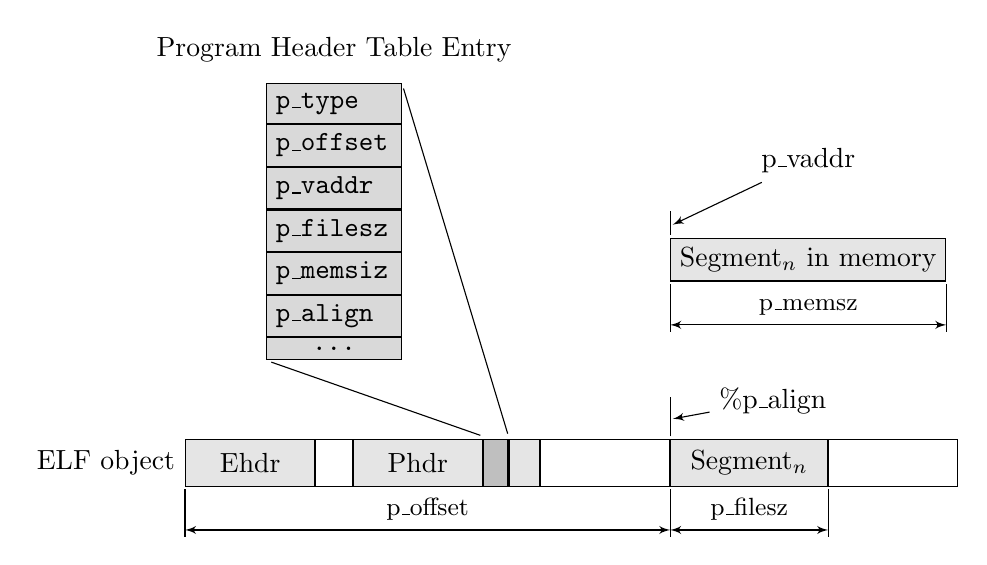
\begin{tikzpicture}[
    start chain=1 going right,
    start chain=2 going above,
    node distance=0pt,
    ef/.style={
      on chain=1,
      draw,
      minimum height=1.4\baselineskip,
      text centered
    },
    ph/.style={
      on chain=2,
      draw,
      text width=4.2em,
      fill=black!15,
      font=\ttfamily
    }]

    % Helper macros.
    \def\l#1#2#3{ \draw[-] ([yshift=#2] #1) -- +(90:#3) }
    \def\sz#1#2#3#4{
        \draw[<->] ([yshift=#3] #1) -- node [auto] {\small #4 }
          ([yshift=#3] #2)
        }

    % Draw a ELF object with a highlighted PHDR entry.
    \node[on chain=1,text width=5 em] {ELF object};
    \node[ef,text width=4em,fill=black!10] (ehdr) {Ehdr};
    \node[ef,text width=1.5ex] (g0) {};
    \node[ef,text width=4em,fill=black!10] (Phdr) {Phdr};
    \node[ef,text width=0.5ex,fill=black!25] (p0) { };
    \node[ef,text width=1ex,fill=black!10] (p1) { };
    \node[ef,text width=4em] (g1) {};
    \node[ef,text width=5em,fill=black!10] (seg)
      {Segment${}_n$};
    \node[ef,text width=4em] (shdr) {};

    % Draw the marks and label sizes and offsets.
    \l{ehdr.south west}{-1pt}{-0.6cm};
    \l{seg.south west}{-1pt}{-0.6cm};
    \l{seg.south east}{-1pt}{-0.6cm};
    \l{seg.north west}{1pt}{0.5cm};
    \node[above right=0.2cm and .5cm of seg.north west] {\%p\_align}
      edge[->,shorten >=1pt] ([yshift=0.25cm] seg.north west);

    \sz{ehdr.south west}{seg.south west}{-0.55cm}{p\_offset};
    \sz{seg.south west}{seg.south east}{-0.55cm}{p\_filesz};

    % Draw the segment in memory.
    \node[above right=2cm and 0cm of seg.north west,draw,fill=black!10]
      (segmem) {Segment${}_n$ in memory};
    \l{segmem.north west}{1pt}{0.3cm};
    \node[above=2em of segmem.north] {p\_vaddr}
      edge [->,shorten >=1pt] ([yshift=0.15cm] segmem.north west);
    \l{segmem.south west}{-1pt}{-0.6cm};
    \l{segmem.south east}{-1pt}{-0.6cm};
    \sz{segmem.south west}{segmem.south east}{-0.55cm}{p\_memsz};

    % Draw the expanded segment.
    \node[ph,above=1cm of g0.north,text centered] (phbot) {\dots};
    \node[ph] {p\_align};
    \node[ph] {p\_memsiz};
    \node[ph] {p\_filesz};
    \node[ph] {p\_vaddr};
    \node[ph] {p\_offset};
    \node[ph] (phtop) {p\_type};

    \node[above=1ex of phtop.north] {Program Header Table Entry};

    % Draw the expansion lines.
    \draw [-,shorten >=1pt,shorten <=2pt] (phbot.south west) --
      ([yshift=1pt] p0.north west);
    \draw [-,shorten >=1pt,shorten <=2pt] (phtop.north east) --
      ([yshift=1pt] p0.north east);

  \end{tikzpicture}
  \caption{ELF Segment Placement.}\label{fig.elf.phdr.layout}
\end{figure}

\begin{callout}{phdr}
  \begin{table}[H]
    \begin{tabular}{rl|ll}
      \mbox{} & \tableheader{32 bit PHDR Table Entry} &
      \tableheader{64 bit PHDR Table Entry}\\ \hline
       & \verb+typedef struct {+&
         \verb+typedef struct {+\\
\co{1} & \verb+  Elf32_Word    p_type;+&
         \verb+  Elf64_Word    p_type;+&\\
\co{2} & \verb+  Elf32_Off     p_offset;+&
         \verb+  Elf64_Word    p_flags;+&\\
\co{3} & \verb+  Elf32_Addr    p_vaddr;+&
         \verb+  Elf64_Off     p_offset;+&\\
\co{4} & \verb+  Elf32_Addr    p_paddr;+&
         \verb+  Elf64_Addr    p_vaddr;+&\\
\co{5} & \verb+  Elf32_Word    p_filesz;+&
         \verb+  Elf64_Addr    p_paddr;+&\\
\co{6} & \verb+  Elf32_Word    p_memsz;+&
         \verb+  Elf64_Xword   p_filesz;+&\\
\co{7} & \verb+  Elf32_Word    p_flags;+&
         \verb+  Elf64_Xword   p_memsz;+&\\
\co{8} & \verb+  Elf32_Word    p_align;+&
         \verb+  Elf64_Xword   p_align;+&\\
       & \verb+} Elf32_Phdr;+ & \verb+} Elf64_Phdr;+&\\
    \end{tabular}
    \caption{ELF Program Header Table Entries.}\label{src.elf.phdr}
  \end{table}

  \begin{description}
  \item[\coref{1}] The \parameter{p\_type} member of the program
    specifies the type of the ELF segment.\index{segments!type} The
    type of the segment is specified by one of the \code{PT\_*}
    constants in the programming API.  Examples include:
    \begin{itemize}
    \item A segment of type \constant{PT\_LOAD} contains data that
      needs to be placed in memory.
    \item A segment of type \constant{PT\_PHDR} describes the ELF
      \elfdatastructure{Program Header Table} itself.
    \item A segment of type \constant{PT\_INTERP} contains a path to
      the runtime linker used by dynamically linked executables.
    \item A segment of type \constant{PT\_NOTE} contains auxiliary
      information.
    \end{itemize}

  \item[\coref{2}] The \parameter{p\_offset} member holds the offset
    from the start of the ELF object to the start of the segment being
    described by this table entry.\index{segments!offset in object}

  \item[\coref{3}] The \parameter{p\_vaddr} member specifies the
    virtual address that this segment should be placed
    at.\index{segments!virtual address of}

  \item[\coref{4}] The \parameter{p\_paddr} member specifies the
    physical memory address this segment should be loaded at.

  \item[\coref{5}] The \parameter{p\_filesz} member specifies the size
    of the segment in the file.  This number can be zero if the
    segment does not use data from file (for example, if the segment
    is a memory-only segment).\index{segments!file size of}

  \item[\coref{6}] The \parameter{p\_memsz} member specifies the
    number of bytes of memory the segment would use.%
    \index{segments!memory size of}

  \item[\coref{7}] The \parameter{p\_flags} member specifies
    additional segment properties.  For example, the value
    \constant{PF\_X} specifies that the segment should be made
    executable, the value \constant{PF\_W} specifies that the segment
    should be writable, and so on.\index{segments!flags}

  \item[\coref{8}] The \parameter{p\_align} member specifies the
    alignment requirements of the segment in memory and in the file.
    This member holds a number that is a power of two.
    \index{segments!aligment of}
  \end{description}
\end{callout}

The file representation of a \elfdatastructure{Program Header Table}
uses the ELF object's native endianness. The \library{libelf} library
will handle the translation between the in-file and in-memory
representations of program header table entries for you. Please see
section~\vref{sec.representations} for more information on in-memory
and in-file representations of ELF data structures.

\section{Example: Reading a Program Header Table}

Let us write a program to print out the program header table in an ELF
object. We will continue to use the ELF class agnostic GELF(3) APIs
in this example.\index{ELF!class~agnostic~APIs}

\begin{callout}{prog3}
  \lstinputlisting[caption=Program 3, label=src.prog.3]{prog3.txt}
  
  \begin{description}
  \item[\coref{1}] Source code that uses the GELF(3) functions needs
    to include the \filename{gelf.h} header file.
  \item[\coref{2}] We define a helper function that translates the
    value of the \parameter{p\_type} member to human-readable form.
  \item[\coref{3}] The GELF(3) functions in this example will use the
    \type{GElf\_Phdr} C type. This type has members that are large
    enough for both the 32-bit (\type{Elf32\_Phdr}) and 64-bit
    (\type{Elf64\_Phdr}) header table
    entries.\index{ELF!class~agnostic~APIs}
  \item[\coref{4}] The function \function{elf\_getphdrnum} will
    retrieve the number of program header table entries in the ELF
    object. However, not every ELF object contains a program header
    table.  We only proceed if a \elfdatastructure{Program Header
      Table} is present.\index{program~header~table!retrieval of}
  \item[\coref{5}] We iterate over the valid indices for the
    \elfdatastructure{Program Header Table} using a C \code{for}
    loop.
  \item[\coref{6}] The \function{gelf\_getphdr} function retrieves the
    program header table entry at a specified index.
    \index{program~header~table!iteration over} If successful it will
    return the \type{GElf\_Phdr} pointer that was passed to it.
  \item[\coref{7}] We then print out the contents of the returned
    \type{GElf\_Phdr} entry.
  \end{description}
\end{callout}

Save the program in listing~\vref{src.prog.3} to file \filename{prog3.c} and
then compile and run it as shown in listing~\vref{scr.prog3}.%
\index{libelf@\texttt{libelf}!linking with}

\begin{callout}{scr3}
  \begin{lstlisting}[language={}, basicstyle=\small\ttfamily,
      label=scr.prog3, caption=Compiling and Running prog3]
% cc -o prog3 prog3.c -lelf @\co{1}@
% ./prog3 prog3 @\co{2}@
PHDR 0:
    p_type               0x6 "PHDR" @\co{3}@
    p_offset             0x34
    p_vaddr              0x8048034
    p_paddr              0x8048034
    p_filesz             0xc0
    p_memsz              0xc0
    p_flags              0x5 [ execute read ]
    p_align              0x4
PHDR 1:
    p_type               0x3 "INTERP" @\co{4}@
    p_offset             0xf4
    p_vaddr              0x80480f4
    p_paddr              0x80480f4
    p_filesz             0x15
    p_memsz              0x15
    p_flags              0x4 [ read ]
    p_align              0x1
PHDR 2:
    p_type               0x1 "LOAD" @\co{5}@
    p_offset             0x0
    p_vaddr              0x8048000
    p_paddr              0x8048000
    p_filesz             0xe67
    p_memsz              0xe67
    p_flags              0x5 [ execute read ]
    p_align              0x1000
PHDR 3:
    p_type               0x1 "LOAD" @\co{6}@
    p_offset             0xe68
    p_vaddr              0x8049e68
    p_paddr              0x8049e68
    p_filesz             0x11c
    p_memsz              0x13c
    p_flags              0x6 [ read write ]
    p_align              0x1000
PHDR 4:
    p_type               0x2 "DYNAMIC"
    p_offset             0xe78
    p_vaddr              0x8049e78
    p_paddr              0x8049e78
    p_filesz             0xb8
    p_memsz              0xb8
    p_flags              0x6 [ read write ]
    p_align              0x4
PHDR 5:
    p_type               0x4 "NOTE"
    p_offset             0x10c
    p_vaddr              0x804810c
    p_paddr              0x804810c
    p_filesz             0x18
    p_memsz              0x18
    p_flags              0x4 [ read ]
    p_align              0x4
  \end{lstlisting}

  \begin{description}
  \item[\coref{1}] Compile and link the program with \library{libelf},
    as before.
  \item[\coref{2}] We run our program on itself, and print out its own
    program header table.  This listing was generated on an i386\trade
    machine running FreeBSD\trade.
  \item[\coref{3}] The very first entry of this program header table
    describes the \elfdatastructure{Program Header Table} itself.%
    \index{program~header~table!self-description}
  \item[\coref{4}] The program \tool{prog3} contains a header entry of
    type \constant{PT\_INTERP} because it is dynamically linked.  A
    segment of type \constant{PT\_INTERP} contains the path name to
    the ``interpreter'' that the kernel should use when executing the
    program.  This is usually the runtime loader (the file
    \filename{/libexec/ld-elf.so.1} on FreeBSD systems).
  \item[\coref{5} \coref{6}] This object contains two loadable
    segments. The first segment requires execute and read permissions,
    and the second read and write permissions.  Both segments require
    page (4096 byte) alignment.\index{segments!examples of}
  \end{description}
\end{callout}

You should try runing \tool{prog3} on other object files.

\begin{itemize}
\item Try running \tool{prog3} on a relocatable object created by a
  \tool{cc -c} invocation.  Does this object have a program header
  table?
\item Try running \tool{prog3} on a shared library.  What does the
  \elfdatastructure{Program Header Table} look like for a shared
  library?
\item Can you find ELF objects on your system that contain program
  header table entries of type \constant{PT\_TLS}?
\end{itemize}

\chapter{Looking at Sections}\label{chap.elf-sections}

Compilers and linkers view ELF objects differently than operating
systems do. These tools treat ELF files as a collection of ELF
\elfdatastructure{Sections}.

An ELF \elfdatastructure{Section}\index{sections} is contiguous region
of an ELF object holding one kind of data. For example, an ELF
relocatable object could have sections with executable code, symbol
tables, code relocation entries, and so on.\index{sections!use~of}
Non-empty sections do not overlap in the ELF object.

\section{The Section Header Table}

The sections of an ELF object are described by a data structure known
as the ELF \elfdatastructure{Section Header Table}.  The
\elfdatastructure{Section Header Table} is usually found at
the very end of the ELF object (see figure~\vref{fig.elf.layout}).
The \parameter{e\_shoff} member in the ELF
\elfdatastructure{Executable Header} for the object specifies the
location of the \elfdatastructure{Section Header Table}.

Every ELF \elfdatastructure{Section} present in an ELF object is
described by an ELF \elfdatastructure{Section Header Table Entry} (see
table~\vref{src.elf.shdr}). Figure~\vref{fig.elf.shdrlayout} shows how
the fields of an ELF \elfdatastructure{Section Header Entry} specify
the section's placement within the ELF
object.\index{sections!placement in file}

\begin{figure}
  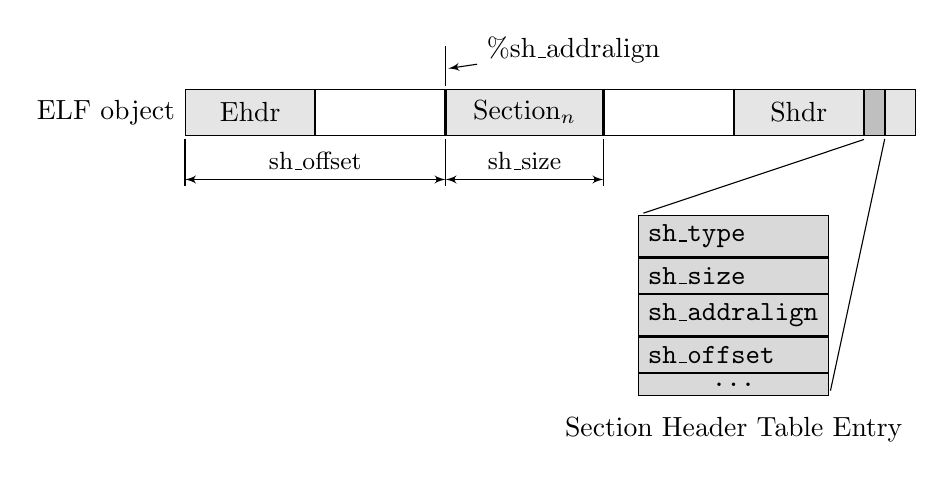
\begin{tikzpicture}[
    start chain=1 going right,
    start chain=2 going below,
    node distance=0pt,
    ef/.style={
      on chain=1,
      draw,
      minimum height=1.4\baselineskip,
      text centered
    },
    sh/.style={
      on chain=2,
      draw,
      text width=6.2em,
      fill=black!15,
      font=\ttfamily
    }]

    % Helper macros.
    \def\l#1#2#3{ \draw[-] ([yshift=#2] #1) -- +(90:#3) }
    \def\sz#1#2#3#4{
        \draw[<->] ([yshift=#3] #1) -- node [auto] {\small #4 }
          ([yshift=#3] #2)
        }

    % Draw a ELF object with a highlighted SHDR entry.
    \node[on chain=1,text width=5 em] {ELF object};
    \node[ef,text width=4em,fill=black!10] (ehdr) {Ehdr};
    \node[ef,text width=4em] (g0) {};
    \node[ef,text width=5em,fill=black!10] (sec)
      {Section${}_n$};
    \node[ef,text width=4em] (g1) {};
    \node[ef,text width=4em,fill=black!10] (shdr) {Shdr};
    \node[ef,text width=0.1ex,fill=black!25] (sh0) { };
    \node[ef,text width=1ex,fill=black!10] {};

    % Draw the marks and label sizes and offsets.
    \l{ehdr.south west}{-1pt}{-0.6cm};
    \l{sec.south west}{-1pt}{-0.6cm};
    \l{sec.north west}{1pt}{0.5cm};
    \l{sec.south east}{-1pt}{-0.6cm};

    \node[above right=0.2cm and 0.4cm of sec.north west] {\%sh\_addralign}
      edge [->,shorten >=1pt] ([yshift=0.25cm] sec.north west);
    \sz{ehdr.south west}{sec.south west}{-0.55cm}{sh\_offset};
    \sz{sec.south west}{sec.south east}{-0.55cm}{sh\_size};

    % Draw the expanded section header entry.
    \node[sh,below=1cm of g1.south east] (shtop) {sh\_type};
    \node[sh] {sh\_size};
    \node[sh] {sh\_addralign};
    \node[sh] {sh\_offset};
    \node[sh,text centered] (shbot) {\dots};
    \node[below=1ex of shbot.south] {Section Header Table Entry};

    % Draw the expansion lines.
    \draw [-,shorten <=2pt] (shtop.north west) --
      ([yshift=-1.2pt] sh0.south west);
    \draw [-,shorten <=2pt] (shbot.south east) --
      ([yshift=-1pt] sh0.south east);
  \end{tikzpicture}
  \caption{Section layout.}\label{fig.elf.shdrlayout}
\end{figure}

\begin{callout}{shdr}
  \begin{table}[H]
    \begin{tabular}{rl|l}
      \mbox{} & \tableheader{32 bit SHDR Table Entry} &
      \tableheader{64 bit SHDR Table Entry} \\ \hline
       & \verb+typedef struct {+ & \verb+typedef struct {+ \\
\co{1} & \verb+  Elf32_Word   sh_name;+&
         \verb+  Elf64_Word   sh_name;+\\
\co{2} & \verb+  Elf32_Word   sh_type;+&
         \verb+  Elf64_Word   sh_type;+\\
\co{3} & \verb+  Elf32_Xword  sh_flags;+&
         \verb+  Elf64_Xword  sh_flags;+\\
       & \verb+  Elf32_Addr   sh_addr;+&
         \verb+  Elf64_Addr   sh_addr;+\\
       & \verb+  Elf32_Off    sh_offset;+&
         \verb+  Elf64_Off    sh_offset;+\\
\co{4} & \verb+  Elf32_Xword  sh_size;+&
         \verb+  Elf64_Xword  sh_size;+\\
\co{5} & \verb+  Elf32_Word   sh_link;+&
         \verb+  Elf64_Word   sh_link;+\\
\co{6} & \verb+  Elf32_Word   sh_info;+&
         \verb+  Elf64_Word   sh_info;+\\
\co{7} & \verb+  Elf32_Word   sh_addralign;+&
         \verb+  Elf64_Word   sh_addralign;+\\
\co{8} & \verb+  Elf32_Word   sh_entsize;+&
         \verb+  Elf64_Word   sh_entsize;+\\
       & \verb+} Elf32_Shdr;+ & \verb+} Elf64_Shdr;+ \\
    \end{tabular}
    \caption{ELF Section Header Table Entries.}\label{src.elf.shdr}
  \end{table}

  \begin{description}
  \item[\coref{1}] The \parameter{sh\_name} member encodes the
    section's name.\index{sections!names} Because section names can be
    of variable length, they are not kept in the section header table
    entry itself.\index{sections!names!as offsets} Instead, all
    section names are placed in a common ``section name string
    table'', and the \parameter{sh\_name} member in the section header
    entry stores the byte offset of the section's name in that string
    table.  The ELF \elfdatastructure{Executable Header} has an
    \parameter{e\_shstrndx} member that contains the section index of
    the section name string table itself.%
    \index{sections!names!string~table} We will look at ELF string
    tables in greater detail in section~\vref{sec.shdr.strtab}.

  \item[\coref{2}] The \parameter{sh\_type} member specifies the
    section's type.  Section types are defined by the
    \code{SHT\_*} constants defined in the system's ELF headers.
    For example, a section of type \constant{SHT\_PROGBITS} would
    contain executable code, and a section of type
    \constant{SHT\_SYMTAB} would hold a symbol
    table.\index{sections!type}

  \item[\coref{3}] The flags field indicates whether the section has
    specific properties; for example, whether it contains writable
    data, whether it has special link ordering requirements, and so
    on.\index{sections!flags}

  \item[\coref{4}] The \parameter{sh\_size} member specifies the size
    of the section in bytes.\index{sections!size of}

  \item[\coref{5} \coref{6}] The \parameter{sh\_link} and
    \parameter{sh\_info} members contain additional section-specific
    information. We do not look at these members further in this
    tutorial.

  \item[\coref{7}] For sections with specific alignment requirements,
    the \parameter{sh\_addralign} member holds the required alignment.
    Its value would be a power of two.\index{sections!alignment of}

  \item[\coref{8}] For sections that contain arrays of fixed-size
    elements, the \parameter{sh\_entsize} member specifies the size of
    each element.\index{section~header~table!entry size}
  \end{description}
\end{callout}


There are a couple of quirks to keep mind when handling ELF sections:

\begin{itemize}
\item First, the section header table entry at index `0'
  (\constant{SHN\_UNDEF}) is special: it is always of type
  \constant{SHT\_NULL}.  When extended numbering is not in use this
  entry has its members set to zero.  When extended numbering is in
  use, the fields of this entry could be non-zero; please see
  section~\vref{sec.extended-numbering} for a discussion on extended
  numbering.\index{sections!indices}

\item Next, valid section indices range from \constant{SHN\_UNDEF} (0)
  up to $\constant{SHN\_LORESERVE} - 1$ (0xFEFF).  Section indices
  between 0xFF00 (\constant{SHN\_LORESERVE}) and 0xFF\-FF
  (\constant{SHN\_HIRESERVE}) have special meanings.  If an ELF object
  has more than 65279 (0xFEFF) sections, then it will need to use
  extended section numbering.\index{sections!indices!valid~indices}
\end{itemize}

\section{ELF Section Handling With \library{libelf}}

The \library{libelf} library offers APIs to retrieve section header
table entries and the contents of sections.\footnote{We will cover the
  adding new sections to ELF objects in
  chapter~\vref{chap.creating-elf}.} These APIs take care of
translating between the in-file and in-memory representations of data
in the ELF object; your application can then directly work with the
in-memory representation of data.%
\index{object~representation!automatic translation}

ELF sections are represented by \library{libelf} using a type named
\type{Elf\_Scn}. This type is meant to be opaque to application
code---the only way to allocate an \type{Elf\_Scn} is by calling one
of \library{libelf}'s APIs.\index{Elf\_Scn@\texttt{Elf\_Scn}!allocation}.

Notable functions in the API that operate on sections include:

\begin{itemize}
\item The function \function{elf\_getscn} retrieves section
  information for a specified section index.%
  \index{sections!retrieval}
\item The function \function{elf\_nextscn} is used to iterate through
  the sections in the ELF object.\index{sections!iteration over}.
\item The function \function{gelf\_getshdr} retrieves the section
  header table entry for a section.%
  \index{section~header~table!retrieval of}
\item The functions \function{elf\_getdata} retrieves the contents of
  the section.
\end{itemize}

\begin{figure}
  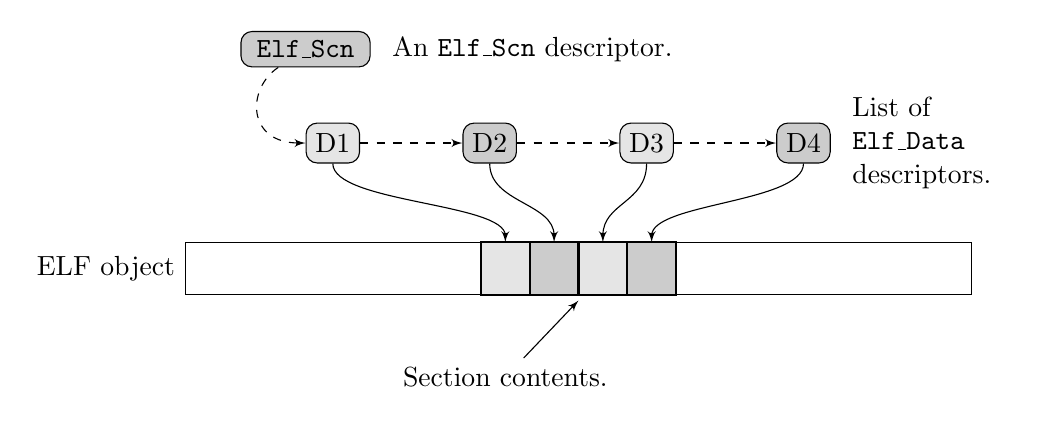
\begin{tikzpicture}[
    start chain=1 going right,
    start chain=2 going right,
    ed/.style={
      on chain=2,
      rectangle,
      rounded corners,
      minimum height=1.2\baselineskip,
      draw,
      node distance=0.5cm,
      fill=black!#1,
      text centered
    },
    eh/.style={
      on chain=1,
      minimum width=4ex,
      text height=\baselineskip,
      draw
    }]

    % Draw the ELF structure.
    \begin{scope}[
      node distance=0pt
      ]
      \node[on chain=1] {ELF object};
      \node[eh,text width=10em] (s0) {};
      \node[eh,fill=black!10] (f0) {};
      \node[eh,fill=black!20] (f1) {};
      \node[eh,fill=black!10] (f2) {};
      \node[eh,fill=black!20] (f3) {};
      \node[eh,text width=10em] {};

      % Highlight the border of the section.
      \draw[-,thick] (f0.north west) -- (f3.north east) --
        (f3.south east) -- (f0.south west) -- cycle;

      % Label the section.
      \node[below=.8cm of f0.south]
        {Section contents.} edge [->] ([yshift=-2pt] f1.south east);
    \end{scope}

    % Draw a linked list of descriptors.
    \begin{scope}[
      node distance=1.3cm,
      every join/.style={->,dashed},
      every on chain/.style={join}
      ]
      \node[ed=10,above=1cm and -1cm of s0.north] (d0) {D1};
      \node[ed=20] (d1) {D2};
      \node[ed=10] (d2) {D3};
      \node[ed=20] (d3) {D4};

      \node[right=1ex of d3,text width=6em]
        {List of \texttt{Elf\_Data} descriptors.};
    \end{scope}

    % Depict an Elf_Scn descriptor referencing the list of descriptors.
    \node[above=0.7cm and -1cm of d0.north west,draw,rounded corners,
      fill=black!20,text width=4em,text centered]
      (scn) {\texttt{Elf\_Scn}};
    \node[right=1ex of scn] {An \texttt{Elf\_Scn} descriptor.};
    \draw[->,dashed,bend right] (scn) .. controls +(-0.75,-0.5) and
      +(-0.75,0) .. (d0.west);

    % Link the Elf_Data descriptors to their section contents.
    \foreach \s in {0,1,2,3} {
      \draw[->] (d\s.south) .. controls +(0,-0.5) and +(0,0.5)
        .. (f\s.north);
    }
  \end{tikzpicture}
  \caption{Coverage of an ELF section by \texttt{Elf\_Scn} and
    \texttt{Elf\_Data} descriptors.}\label{fig.elf.scn}
\end{figure}

An \type{Elf\_Scn} descriptor is associated with zero or more
\type{Elf\_Data} descriptors. Each \type{Elf\_Data} descriptor
describes a region of application memory containing data for the ELF
section. Figure~\vref{fig.elf.scn} shows how the \type{Elf\_Data}
descriptors for an \type{Elf\_Scn} descriptor could cover the content
of a section.\index{sections!coverage by data descriptors}

Listing~\vref{fig.elf.scn-data.decl} shows the C definition of the
\type{Elf\_Scn} and \type{Elf\_Data} types.

\begin{callout}{data}
  \begin{lstlisting}[caption=The \type{Elf\_Data} and \type{Elf\_Scn} types,
      label=fig.elf.scn-data.decl, basicstyle=\small\ttfamily]
typedef struct _Elf_Scn Elf_Scn;   @\co{1}@
typedef struct _Elf_Data {
        /*
         * `Public' members that are part of the ELF(3) API.
         */
        uint64_t        d_align;   @\co{2}@
        void            *d_buf;    @\co{3}@
        uint64_t        d_off;     @\co{4}@
        uint64_t        d_size;    @\co{5}@
        Elf_Type        d_type;    @\co{6}@
        unsigned int    d_version; @\co{7}@
        /* ... other library-private fields ... */
} Elf_Data;
  \end{lstlisting}

  \begin{description}
  \item[\coref{1}] The \type{Elf\_Scn} type is opaque to the
    application.
  \item[\coref{2}] The \parameter{d\_align} member specifies the
    alignment of the data referenced in the \type{Elf\_Data} with
    respect to its containing section.%
    \index{Elf\_Data@\texttt{Elf\_Data}!alignment}
  \item[\coref{3}] The \parameter{d\_buf} member points to a contiguous
    region of application memory containing the section's data.%
    \index{Elf\_Data@\texttt{Elf\_Data}!data pointer}
  \item[\coref{4}] The \parameter{d\_off} member contains the file
    offset from the start of the section for the data in this buffer.
    \index{Elf\_Data@\texttt{Elf\_Data}!offset in section}
  \item[\coref{5}] The \parameter{d\_size} member contains the size of
    the memory buffer in bytes.%
    \index{Elf\_Data@\texttt{Elf\_Data}!data size}
  \item[\coref{6}] The \parameter{d\_type} member specifies the ELF
    type of the data contained in the data buffer.  Legal values for
    this member are defined by the \type{Elf\_Type}
    enumeration in the \filename{libelf.h} header file.%
    \index{Elf\_Data@\texttt{Elf\_Data}!data type}
  \item[\coref{7}] The \parameter{d\_version} member specifies the
    working version for the data in this descriptor.  It must be one
    of the values supported by the \library{libelf} library.%
    \index{Elf\_Data@\texttt{Elf\_Data}!descriptor version}
    Please see chapter~\ref{chap.getting-started} for more information on
    ELF version numbers.
  \end{description}
\end{callout}

Figure~\vref{fig.elf.data} shows how the members of the
\type{Elf\_Data} descriptor describe a region of application memory
containing section data. As seen in the figure, the in-memory
representation of this data might have a different size and different
endianness than its in-file
representation.\index{Elf\_Data@\texttt{Elf\_Data}!describing application
  memory}

\begin{figure}
  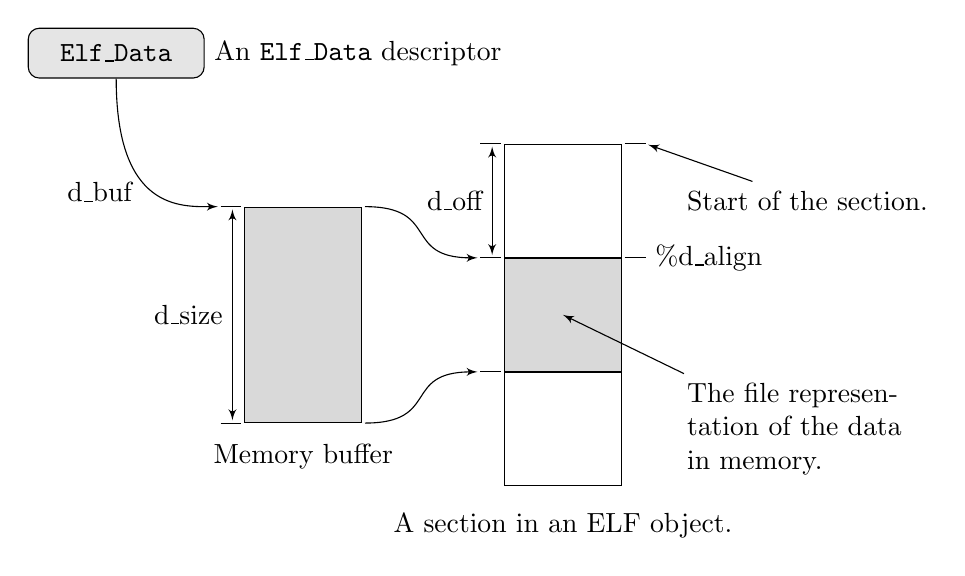
\begin{tikzpicture}[
    eh/.style={
      text width=1.25cm,
      text height=1.2cm,
      draw
    }]

    \node[text width=2cm,minimum height=1.5\baselineskip,font=\ttfamily,
      draw,rounded corners,fill=black!10,text centered]
      (data) {Elf\_Data};
    \node[node distance=0pt,right=of data] {An \texttt{Elf\_Data} descriptor};

    % Draw the memory representation of the data.
    \node[below right=2.3cm of data.south,text width=1.25cm,text height=2.5cm,
      draw,fill=black!15] (mem) {};
    % .. and label it.
    \node[below=1ex of mem.south] {Memory buffer};

    % Place tick marks.
    \coordinate (a0) at ([xshift=-0.3cm] mem.north west);
    \coordinate (a1) at ([xshift=-0.3cm] mem.south west);

    \draw[-,shorten >=1pt] (a0) -- (mem.north west);
    \draw[-,shorten >=1pt] (a1) -- (mem.south west);
    \draw[<->,shorten >=1pt,shorten <=1pt] ([xshift=0.15cm] a0) --
      ([xshift=0.15cm] a1) node [midway,left] {d\_size};

    % Link the Elf_Data descriptor to the memory buffer.
    \draw[->,bend right=45,shorten >=1pt] (data) .. controls +(0,-2)
      and +(-.5,0) .. (a0) node[left=1ex,midway] {d\_buf};

    % Draw the ELF object.
    \begin{scope}[
      node distance=0pt
      ]
      \node[eh,right=1.8cm of mem,fill=black!15] (e1) {};
      \node[eh,above=of e1] (e0) {};
      \node[eh,below=of e1] (e2) {};
    \end{scope}

    % Label the ELF object.
    \node[below=1.5ex of e2.south] {A section in an ELF object.};

    % Place tick marks and the d_align label.
    \foreach \c in {0,1,2} {
      \coordinate (b\c) at ([xshift=-.3cm] e\c.north west);
      \draw[-,shorten >=1pt] (b\c) -- (e\c.north west);
    };

    \draw[-,shorten <=1pt] (e0.north east) -- +(.3cm,0);
    \draw[-,shorten <=1pt] (e1.north east) -- +(.3cm,0)
      node[right] {\%d\_align};

    % Place other labels.
    \node[right=2em of e0.east] {Start of the section.}
      edge [->,shorten >=1pt] ([xshift=.3cm] e0.north east);

    \draw[<->,shorten >=1pt,shorten <=1pt] ([xshift=.15cm] b0) --
      ([xshift=.15cm] b1) node [midway,left] {d\_off};

    \node[right=2em of e2.east,text width=8em]
      {The file representation of the data in memory.}
      edge [->] (e1.center);

    % Link the memory and file representations.
    \draw[->,shorten >=1pt,shorten <=1pt] (mem.north east) .. controls +(1,0)
      and +(-1,0) .. (b1);
    \draw[->,shorten >=1pt,shorten <=1pt] (mem.south east) .. controls +(1,0)
      and +(-1,0) .. (b2);
  \end{tikzpicture}
  \caption{How \type{Elf\_Data} descriptors work.}\label{fig.elf.data}
\end{figure}

\section{ELF String Tables}\label{sec.shdr.strtab}

Before we can proceed to our example program for the chapter we need
to understand how ELF string tables are structured.

ELF string tables hold variable length strings.  Other ELF data
structures refer to the strings stored in these tables by using byte
offsets from the start of each string table.

\begin{figure}
  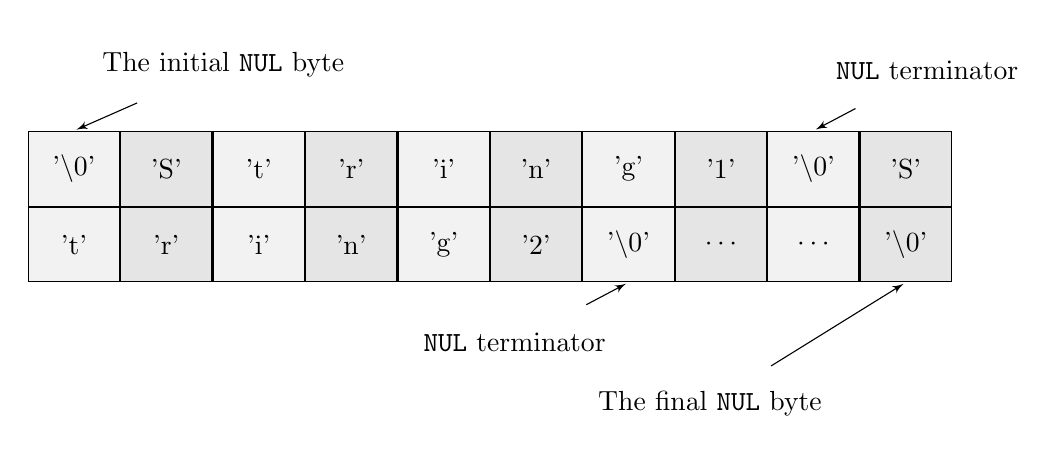
\begin{tikzpicture}[
    rectangle,
    node distance=0pt,
    minimum size=2.7em,
    minimum width=3.3em,
    inner sep=0pt,
    se/.style={
      draw,
      fill=black!5
    },
    so/.style={
      draw,
      fill=black!10
    }]

    % Draw the string table.
    \matrix [row sep=0pt, column sep=0pt] {
        \node[se] (n0) {'\textbackslash 0'}; & \node[so] {'S'}; &
        \node[se] {'t'}; &                \node[so] {'r'}; &
        \node[se] {'i'}; &                \node[so] {'n'}; &
        \node[se] {'g'}; &                \node[so] {'1'}; &
        \node[se] (n1) {'\textbackslash 0'}; & \node[so] {'S'}; \\
        \node[se] {'t'}; & \node[so] {'r'}; &
        \node[se] {'i'}; & \node[so] {'n'}; &
        \node[se] {'g' }; & \node[so] {'2'}; &
        \node[se] (n2) {'\textbackslash 0'}; & \node[so] {$\cdots$}; &
        \node[se] {$\cdots$}; & \node[so] (n3) {'\textbackslash 0' };\\
      };

    % Add labels.
    \def\N{\texttt{NUL}\xspace}
    \node[above right=0.5cm of n0.north] {The initial \N byte}
      edge [->,shorten >=1pt] (n0.north);

    \node[above right=0.4cm of n1.north]
      {\N terminator} edge [->,shorten >=1pt] (n1.north);

    \node[below left=0.4cm of n2.south] {\N terminator}
      edge [->,shorten >=1pt] (n2.south);

    \node[below left=1.5cm of n3.south] {The final \N byte}
      edge [->,shorten >=1pt] (n3.south);
  \end{tikzpicture}
  \caption{String Table Layout.}\label{fig.elf.strtab}
\end{figure}

Figure~\vref{fig.elf.strtab} shows the layout of a string table.%
\index{string~tables!layout}

\begin{itemize}
\item The initial byte of a string table is \code{NUL} (a
  `\(\backslash\)0').  This allows a string offset value of zero to
  denote the empty string.
\item Subsequent strings are separated by \code{NUL} bytes.
\item The final byte in the section is a \code{NUL}, in order to
  \code{NUL}-terminate the last string in the string table.
\end{itemize}

Sections containing string tables have section type
\constant{SHT\_STRTAB}.

An ELF file can have multiple string tables. For example, the names of
the sections could be kept in a section name string table while the
names of program symbols could be kept in a symbol name string
table.\index{ELF!string tables}

The \function{elf\_strptr} function in the \library{libelf} library
converts string table offsets into \code{char *} pointers usable by
C code.\index{string~tables!retrieval of strings}

\section{Example: Listing Section Names}

Let us now write an example program that retrieves and prints the
names of the sections in an ELF object.

\begin{callout}{prog4}
  \lstinputlisting[caption=Program 4, label=src.prog.4]{prog4.txt}

  \begin{description}
    \item[\coref{1}] We first retrieve and save the section index of
      the section name string table using the function
      \function{elf\_getshdrstrndx}.  Using this function allows our
      program to work correctly when the object being examined uses
      extended numbering.\index{sections!names!string~table}%
      \index{extended number!use of}
    \item[\coref{2}] The function \function{elf\_nextscn} has the
      useful property that it will return the pointer to the
      \type{Elf\_Scn} descriptor for section number 1 if a NULL
      pointer is passed in to it.  Recall that section number 0 is
      always of type \constant{SHT\_NULL}, and is not interesting to
      applications.
    \item[\coref{3}] We loop through the sections in the ELF object.
      Function \function{elf\_nextscn} will return NULL after the last
      section has been traversed; this gives us a convenient way to
      exit our processing loop.
    \item[\coref{4}] Given a pointer to an \type{Elf\_Scn}, we
      retrieve the associated section header table entry using the
      \function{gelf\_getshdr} function.  The \parameter{sh\_name}
      member of the returned section header table entry holds the
      offset of the section's name in the section name string
      table.\index{sections!header table entry}
    \item[\coref{5}] We convert the offset in member
      \parameter{sh\_name} to a \code{char *} pointer using the
      \function{elf\_strptr} function.  We print the section's name
      using \code{printf}.
    \item[\coref{6}] Next, we will print the contents of the section
      name string table itself. We retrieve the \type{Elf\_Scn}
      descriptor for the section name string
      table.\index{sections!names!string~table}
    \item[\coref{7}] We cycle through the \type{Elf\_Data} descriptors
      for the section, printing the characters in each data buffer.
  \end{description}
\end{callout}

Save the program in listing~\vref{src.prog.4} to file
\filename{prog4.c} and then compile and run it as shown in
listing~\vref{scr.prog4}.%
\index{libelf@\texttt{libelf}!linking with}

\begin{callout}{scr4}
  \newcommand{\at}{@}
  \begin{lstlisting}[language={}, basicstyle=\small\ttfamily,
      label=scr.prog4, caption=Compiling and Running prog4]
% cc -o prog4 prog4.c -lelf @\co{1}@
% ./prog4 prog4 @\co{2}@
Section 0001 .interp
Section 0002 .note.ABI-tag
Section 0003 .hash
Section 0004 .dynsym
Section 0005 .dynstr
Section 0006 .rela.plt
Section 0007 .init
Section 0008 .plt
Section 0009 .text
Section 0010 .fini
Section 0011 .rodata
Section 0012 .data
Section 0013 .eh_frame
Section 0014 .dynamic
Section 0015 .ctors
Section 0016 .dtors
Section 0017 .jcr
Section 0018 .got
Section 0019 .bss
Section 0020 .comment
Section 0021 .shstrtab @\co{3}@
Section 0022 .symtab
Section 0023 .strtab
.shstrab: size=287 @\co{4}@
\^@\at@ . s y m t a b \^@\at@ . s t r t a b
\^@\at@ . s h s t r t a b \^@\at@ . i n t e
r p \^@\at@ . h a s h \^@\at@ . d y n s y m
@\ldots{}\textit{etc}\ldots@
  \end{lstlisting}

  \begin{description}
  \item[\coref{1}] Compile and link the program in the standard way.
  \item[\coref{2}] We make our program print the names of its own
    sections.
  \item[\coref{3}] The section name string table is called
    \code{.shstrtab} by convention.
  \item[\coref{4}] This is the content of the section name string table
    itself.
  \end{description}
\end{callout}

\chapter{Creating New ELF Objects}\label{chap.creating-elf}

In this chapter we will use the \library{libelf} library to create a
new ELF object.\index{ELF!creation~of}

\section{Example: Creating an ELF Object}

Listing~\vref{src.prog.5} has an example program that creates an ELF
file with the following content:

\begin{itemize}
\item A section named ``\code{.foo}'' containing data in the form
  of 32-bit words that may need byte-swapping. We had discussed
  \library{libelf}'s handling of data needing byte-swapping in
  section~\vref{sec.representations}.
\item A section named ``\code{.shstrtab}'' containing the section
  name string table for our ELF object. We covered string tables
  in section~\vref{sec.shdr.strtab}.
\item A \elfdatastructure{Program Header Table} with a single
  \elfdatastructure{Program Header Table Entry} covering the program
  header table itself. We studied the ELF \elfdatastructure{Program
    Header Table} in chapter~\ref{chap.elf-phdr}.
\end{itemize}

Our new ELF object will be marked as a 32-bit PowerPC\trade
executable, and will use MSB-first data ordering.

\begin{callout}{prog5}
  \lstinputlisting[caption=Program 5, label=src.prog.5]{prog5.txt}

  \begin{description}
  \item[\coref{1}] The header file \filename{libelf.h} brings in function
    prototypes for \library{libelf}'s functions.

  \item[\coref{2}] The \code{hash\_words} array holds 32-bit
    words. The values in the array would need to be written using
    big-endian byte ordering when the section is written to
    file.\index{sections!hash~values}

  \item[\coref{3}] We will use a pre-fabricated string table
    containing the names of our two sections, ``\code{.foo}'' and
    ``\code{.shstrtab}''.\index{string~tables}

  \item[\coref{4}] The first step in creating a new ELF object is to
    obtain a file descriptor opened for writing from the operating
    system.

  \item[\coref{5}] Next, we obtain an \type{Elf} handle by calling the
    function \function{elf\_begin}. We use the parameter
    \constant{ELF\_C\_WRITE} to inform \library{libelf} of our
    intention to create a brand new ELF
    object.\index{object~creation}

  \item[\coref{6}] We allocate an ELF \elfdatastructure{Executable
    Header} using the function \function{elf32\_newehdr}.  An
    \elfdatastructure{Executable Header} is always needed for an ELF
    object.\index{executable~header!allocation}

    We then populate the executable header:
    \begin{enumerate}
    \item We set the \constant{EI\_DATA} byte in its
      \parameter{e\_ident} member to the desired endianness
      (big-endian in our case).
    \item We set the machine type to the constant \constant{EM\_PPC},
      for the PowerPC\trade architecture.
    \item We mark the object as an ELF executable.
    \end{enumerate}

    Our new object will be a 32-bit object, because we had allocated
    its \elfdatastructure{Executable Header} using the 32-bit
    \function{elf32\_newehdr} function.

  \item[\coref{7}] We allocate an ELF \elfdatastructure{Program Header
    Table} containing a single entry. This entry is meant to cover the
    \elfdatastructure{Program Header Table} itself.

    At this point in our program we do not know the file offset at
    which the ELF \elfdatastructure{Program Header Table} will be
    placed inside our new ELF object.  This offset would only be known
    after the object is laid out.  We need to defer filling in our
    program header table entry until \library{libelf} has computed an
    object layout for us (please see step 11 below).

  \item[\coref{8}] We create an \type{Elf\_Scn} descriptor for the ELF
    section holding the values in the \code{hash\_words} array.

    To actually associate data with our new section we allocate an
    \type{Elf\_Data} descriptor and set its fields to map the
    \code{hash\_words} array.

    A call to \function{elf32\_getshdr} then returns the
    \elfdatastructure{Section Header Table Entry} for the new section.

    \begin{enumerate}
    \item We set the type of the new section to \constant{SHT\_HASH}.
      The \library{libelf} library knows how to byte-swap sections of
      this type.

    \item We mark the section as having content in the file by setting
      its \parameter{sh\_flags} field to the constant
      \constant{SHF\_ALLOC}.
    \end{enumerate}

  \item[\coref{9}] We then allocate another section for holding the
    section name string
    table.\index{string~tables!allocation~of}

    We allocate an \type{Elf\_Data} descriptor for this section, and
    use it to map the pre-fabricated string table in the array
    \code{string\_table}.

    We retrieve the \elfdatastructure{Section Header Table Entry} for
    this section and set its members:

    \begin{enumerate}
    \item The type of our string table section is set to
      \constant{SHT\_STRTAB}, the section type for string tables.
    \item The section flags are set to indicate that the section
      contains data in the file, and that it contains
      \code{NUL}-terminated strings.
    \end{enumerate}

  \item[\coref{10}] We use the function \function{elf\_ndxscn} to
    retrieve the section index for our string table section. We use
    the function \function{elf\_setshstrndx} to set the section name
    string table index field in the ELF \elfdatastructure{Executable
      Header}.\index{executable~header!section name string table}

  \item[\coref{11}] We then ask the \library{libelf} library to
    compute a layout for our ELF object without writing the object
    out.  We do this by calling the function \function{elf\_update}
    with the parameter \constant{ELF\_C\_NULL}.

    Once the call to \function{elf\_update} returns we examine the
    \elfdatastructure{Executable Header} to determine where
    \library{libelf} had placed the \elfdatastructure{Program Header
      Table}. We update the \elfdatastructure{Program Header Table
      Entry} created in step 7 to cover the program header table.

    We then mark the \elfdatastructure{Program Header Table} as
    modified using a call to function \function{elf\_flagdata}.%
    \index{executable~header!updating}

    \item[\coref{12}] Finally, we call function \function{elf\_update}
      with parameter \constant{ELF\_C\_WRITE} to write the ELF object
      out to file.\index{object~creation!writing to file}

      If our example program is run on a little-endian host the
      \library{libelf} library will byte-swap the sections that need
      byte-swapping when the ELF object is written out to file.
  \end{description}
\end{callout}

Save the program in listing~\vref{src.prog.5} to file
\filename{prog5.c} and then compile and run it as shown in
listing~\vref{scr.prog5}.%
\index{libelf@\texttt{libelf}!linking with}

\begin{callout}{scr5}
  \begin{lstlisting}[language={}, basicstyle=\small\ttfamily,
      label=scr.prog5, caption=Compiling and Running prog5]
% cc -o prog5 prog5.c -lelf @\co{1}@
% ./prog5 foo
% file foo @\co{2}@
foo: ELF 32-bit MSB executable, PowerPC or cisco 4500, \
     version 1 (SYSV), statically linked, stripped
% readelf -a foo @\co{3}@
ELF Header:
  Magic:   7f 45 4c 46 01 02 01 00 00 00 00 00 00 00 00 00
  Class:                             ELF32
  Data:                              2's@\,@complement,@\,@big@\,@endian
  Version:                           1 (current)
  OS/ABI:                            UNIX - System V
  ABI Version:                       0
  Type:                              EXEC (Executable file)
  Machine:                           PowerPC
  Version:                           0x1
  Entry point address:               0x0
  Start of program headers:          52 (bytes into file)
  Start of section headers:          112 (bytes into file)
  Flags:                             0x0
  Size of this header:               52 (bytes)
  Size of program headers:           32 (bytes)
  Number of program headers:         1
  Size of section headers:           40 (bytes)
  Number of section headers:         3
  Section header string table index: 2
@\ldots etc\ldots@
  \end{lstlisting}

  \begin{description}
  \item[\coref{1}] Compile, link and run the program as in our
    previous examples.
  \item[\coref{2} \coref{3}] We can use the \tool{file} and
    \tool{readelf} programs to examine the object that we have
    created.
  \end{description}
\end{callout}

\section{Controlling ELF Layout}\label{sec.controlling-layout}
By default, the \library{libelf} library will lay out your ELF objects
for you.  The default layout is shown in
figure~\vref{fig.elf.layout}.\index{object~creation!default~layout}%

You can request fine-grained control over the ELF object's layout by
setting the \constant{ELF\_F\_LAYOUT} flag on its \type{Elf}
descriptor. This flag is set using the function \function{elf\_flagelf}.%
\index{object~creation!application control of layout}

After setting the \constant{ELF\_F\_LAYOUT} flag on an \type{Elf}
descriptor, you can control the layout of the ELF object using the
following parameters:

\begin{itemize}
\item You can set the values of the \parameter{e\_phoff} and
  \parameter{e\_shoff} members of the \elfdatastructure{Executable
    Header}. These values determine where the ELF
  \elfdatastructure{Program Header Table} and
  \elfdatastructure{Section Header Table} would be placed in the ELF
  object.

\item For each section you can set the \parameter{sh\_addralign},
  \parameter{sh\_offset}, and \parameter{sh\_size} members of the
  section's header table entry.  These members control the placement
  of the section within the ELF object.
\end{itemize}

These members must be set prior to calling the \function{elf\_update}
function.

\section{Fill Characters}

The \library{libelf} library will fill the gaps between the parts of
the ELF object with a fill character.\index{ELF!fill character} These
gaps may arise due to the alignment constraints on adjacent sections.

You can set the fill character to use by calling the function
\function{elf\_fill} before calling \function{elf\_update}.  The
default fill character is a zero byte.%
\index{object~creation!fill~character}%

\section{Memory Ownership}

Some of the APIs implemented by \library{libelf} return pointers to
memory arenas; other APIs accept pointers to memory arenas as input.
Knowing when you should (or should not) call \code{free()} on a
pointer is important to avoid corrupting memory.

The \library{libelf} library follows a simple rule: it will not free
data that it did not allocate. Conversely, it \emph{will} free memory
that it had allocated.%
\index{libelf@\texttt{libelf}!API!memory~management~rules}

You should not free pointers returned by \library{libelf}, such as the
\code{Elf\_Scn *} pointers returned by calls to \function{elf\_getscn}
and the \code{Elf\_Data~*} pointers returned by calls to
\function{elf\_newdata}.  Conversely, if you had allocated the memory
arena mapped by an \type{Elf\_Data} structure using \code{malloc()}
or \code{new()}, then you should release the arena once you are done
with it.


\section{Data Structure Lifetimes}

Many of \library{libelf}'s APIs return pointers to its internal data
structures. In objects opened for writing these pointers have a
limited lifetime---they are only valid up till the time the ELF object
is written out to file by a call to function \function{elf\_update}.%
\index{libelf@\texttt{libelf}!API!data structure refresh rules}

This is because when \library{libelf} writes out an ELF object, it
releases and reallocates some of its internal bookkeeping structures.

After calling function \function{elf\_update} with parameter
\constant{ELF\_C\_WRITE} you should treat any prior pointers returned
by \library{libelf}, such as pointers to \type{Elf\_Scn} and
\type{Elf\_Data} structures, as invalid. If you wish to continue
working with your ELF object, you should retrieve these pointers
afresh from \library{libelf}.%
\index{libelf@\texttt{libelf}!API!pointer validity}

\section{Modifying Existing ELF Objects}\label{sec.modifying-elf}

You can use the \library{libelf} library to modify existing ELF
objects.

The process to update an ELF object is similar to that for creating
ELF objects, with the following
differences:\index{object~modification}

\begin{itemize}
\item You would open the underlying file for both reading and writing,
  i.e., with mode \code{O\_RDWR}.

\item You would need an \type{Elf} descriptor that is valid for
  updates.  You can allocate a suitable descriptor by calling function
  \function{elf\_begin} using the parameter \constant{ELF\_C\_RDWR}.

\item You can use functions such as \function{elf\_newscn},
  \function{elf32\_newphdr} and \function{elf64\_newphdr} to add new
  data structures to your object.%
  \index{object~modification!adding new structures}
  You can also retrieve existing ELF data structures in the file using
  APIs such as those discussed in the previous chapters of this
  tutorial.  You can add new data to existing sections using the
  function \function{elf\_newdata}.

\item After you modify the fields of a data structure retrieved from
  the ELF object, you should call the appropriate
  \function{elf\_flag} functions to inform \library{libelf} about
  your change.\index{object~modification!flagging modified data}
\end{itemize}

A caution: when you update an ELF object, you should take care to
ensure that the resulting object remains a valid ELF object. For
example, if you move the sections of an ELF executable around, then
you should also keep the relevant offsets in its
\elfdatastructure{Program Header Table} entries updated. We will not
however explore this topic further in this introductory tutorial.

\chapter{Processing \tool{ar} Archives}\label{chap.ar}

During program development the \tool{ar} archiver is used to manage
``libraries'' of object files.\index{archive library} You can use the
\library{libelf} library to read these archives.

The \library{libelf} library's APIs are `read-only'---we cannot create
new \tool{ar} archives (or modify existing archives) using its APIs.%
\footnote{The
  \href{https://github.com/libarchive/libarchive/wiki}{\library{libarchive}}
  library could be used to create or modify \tool{ar} archives.}

In this chapter we will build an example program that takes an
\tool{ar} archive as input and lists the names and sizes of the files
contained within it.

\section{The Structure of \tool{ar} Archives}

Every \tool{ar} archive starts with a signature sequence of 8 bytes
(please see the constant \constant{ARMAG}\index{ar~archive!magic}
defined in the system header \filename{ar.h}).  The members of the
archive follow this signature.

Figure~\vref{fig.arstr} shows the structure of an
\tool{ar} archive.

\begin{figure}
  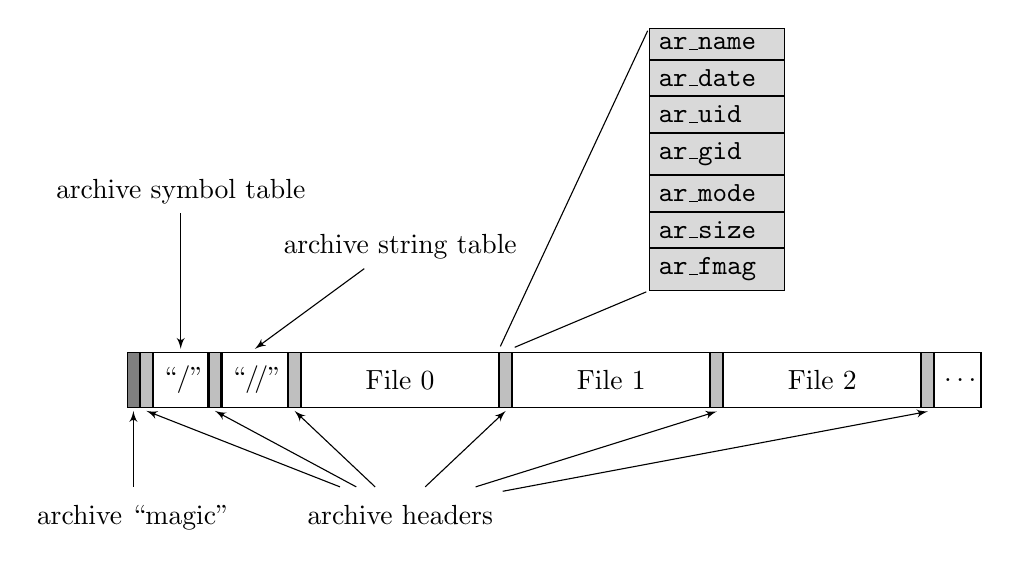
\begin{tikzpicture}[
    file/.style={               % Boxes denoting archive content.
      rectangle,
      draw,
      text centered,
      text width=6.45em,
      node distance=0pt,
      minimum height=2em
    },
    arhdr/.style={             % Boxes denoting archive headers.
      rectangle,
      draw,
      fill=black!25,
      node distance=0pt,
      minimum height=2em,
      minimum width=1ex,
      inner sep=0pt
    },
    lbl/.style={                % Styling of label text.
      text height=1em
    },
    hdr/.style={
      text width=4.2em,
      draw,
      fill=black!15,
      node distance=0pt,
      font=\ttfamily
    }]

    % Depict the structure of the archive.
    \node[arhdr,fill=black!50] (magic) {};
    \node[arhdr] (s0) [right=of magic] {};
    \node[file,text width=1.3em]   (symtab) [right=of s0] {``/''};
    \node[arhdr] (s1) [right=of symtab] {};
    \node[file,text width=1.7em]  (strtab) [right=of s1] {``$/\!/$''};
    \node[arhdr] (h0) [right=of strtab] {};
    \node[file]  (f0) [right=of h0] {File 0};
    \node[arhdr] (h1) [right=of f0] {};
    \node[file]  (f1) [right=of h1] {File 1};
    \node[arhdr] (h2) [right=of f1] {};
    \node[file]  (f2) [right=of h2] {File 2};
    \node[arhdr] (h3) [right=of f2] {};
    \node[file,text width=1em] (f3) [right=of h3] {$\ldots$};

    % Label the elements of the archive.
    \node[lbl] (lmagic) [below=of magic,text height=1em] {archive ``magic''}
      edge [->] ([yshift=-1pt] magic.south);
    \node[lbl] (lheader) [below=of f0.south,text height=1em] {archive headers}
      edge [->] ([yshift=-1pt] s0.south)
      edge [->] ([yshift=-1pt] s1.south)
      edge [->] ([yshift=-1pt] h0.south)
      edge [->] ([yshift=-1pt] h1.south)
      edge [->] ([yshift=-1.2pt] h2.south)
      edge [->] ([yshift=-1.2pt] h3.south);
    \node[lbl] (lsymtab) [above=5em of symtab.north]
      {archive symbol table}
      edge [->] ([yshift=1pt] symtab.north);
    \node[lbl] (lstrtab) [above=3em of f0.north]
      {archive string table}
      edge [->] ([yshift=1pt] strtab.north);

    % Show the internal structure of an archive header.
    \node[hdr] (arfmag) [above=2.2em of h2.north]
        {\texttt{ar\_fmag}};
    \node[hdr] (arsize) [above=of arfmag.north] {ar\_size};
    \node[hdr] (armode) [above=of arsize.north] {ar\_mode};
    \node[hdr] (argid)  [above=of armode.north] {ar\_gid};
    \node[hdr] (aruid)  [above=of argid.north]  {ar\_uid};
    \node[hdr] (ardate) [above=of aruid.north]  {ar\_date};
    \node[hdr] (arname) [above=of ardate.north] {ar\_name};

    % Draw "expansion" lines.
    \draw[shorten >=1pt, shorten <=1pt] ([yshift=1.2pt] h1.north east)
      to (arfmag.south west);
    \draw[shorten >=1pt, shorten <=1pt] ([yshift=1pt] h1.north west)
      to (arname.north west);
  \end{tikzpicture}
  \caption{The structure of \tool{ar} archives.}\label{fig.arstr}
\end{figure}

\subsection{The Archive Header}

Each member of an \tool{ar} archive is preceded by an archive
header\index{ar~archive!header} that describes the member's
attributes. The archive header is a collection of fixed-size ASCII
strings that resides at an even offset within the archive
file.\index{ar~archive!header!layout} Listing~\vref{src.arhdr} shows
the layout of the archive header as a C \code{struct}.

\begin{lstlisting}[caption=Archive Header Layout, label=src.arhdr]
struct ar_hdr {
    char ar_name[16]; /* file name */
    char ar_date[12]; /* file modification time */
    char ar_uid[6];   /* creator user id */
    char ar_gid[6];   /* creator group id */
    char ar_mode[8];  /* octal file permissions */
    char ar_size[10]; /* size in bytes */
#define        ARFMAG   "`\n"
    char ar_fmag[2];  /* consistency check */
} __packed;
\end{lstlisting}

\section{Special Archive Members}
The initial members of an \tool{ar} archive may be special:

\begin{itemize}
\item An archive member with the name ``/'' is an archive symbol
  table\index{ar~archive!symbol~table}.  This symbol table maps
  program symbols to archive members in the archive.  It is usually
  maintained by tools like \tool{ranlib} and \tool{ar}.

\item An archive member with the name ``/\hskip-.2ex/'' is an archive
  string table\index{ar~archive!string~table}.

  The \tool{ar} archive header can only contain fixed size ASCII
  strings. Member file names that exceed the length limits of the
  \parameter{ar\_name} archive header field would need to be placed in
  a special string table.\footnote{Archive string tables are not to be
    confused with ELF string tables. ELF string tables were examined
    in section~\ref{sec.shdr.strtab}.}  The \parameter{ar\_name} field
  of the archive header would then hold the offset within the archive
  string table of the real file name, encoded as a decimal
  number.\index{ar~archive!long~file~names}
\end{itemize}

\section{Archive Flavors}

\tool{ar} archives come in two flavors mainly: BSD and SVR4.  These
flavors are different in many respects---for example, SVR4 archives
use a `/' character to terminate file names in the archive header,
whereas BSD format archives use a ASCII space character as a
terminator.  The way the two formats handle long file names is also
different. The archive handling APIs offered by the \library{libelf}
library will insulate your code from the differences between the
archive formats.

\section{Archive Symbol Tables}\label{sec.ar.symtab}

An archive symbol table helps linkers to quickly locate the ELF
objects in an archive. The BSD and SVR4 archive flavors have their own
archive symbol table formats.

If an archive symbol table is present in an \tool{ar} archive, it will
be the archive's first member.

You can read an \tool{ar} archive's symbol table using the function
\function{elf\_getarsym}.\index{ar~archive!symbol~table!retrieval of}
This function returns an array of \type{Elf\_Arsym} structures, where
each \type{Elf\_Arsym} structure maps a program symbol to a file
offset within the \tool{ar} archive. These file offsets can then be
used with the \function{elf\_rand} function to retrieve the ELF object
in question (please see section~\ref{sec.ar.random-access} below).

Listing~\vref{fig.arsym} contains the C definition of an
\type{Elf\_Arsym} data type.

\begin{lstlisting}[caption=The \type{Elf\_Arsym} structure,
    label=fig.arsym, basicstyle=\small\ttfamily]
typedef struct {
  off_t         as_off;   /* byte offset to member header */
  unsigned long as_hash;  /* elf_hash() value for name */
  char          *as_name; /* null terminated symbol name */
} Elf_Arsym;
\end{lstlisting}

\section{Random Archive Access Using \function{elf\_rand}}
\label{sec.ar.random-access}

Instead of iterating over the members of an \tool{ar} archive in
sequence, you can also directly access specific members in the archive
using the \function{elf\_rand}
function.\index{ar~archive!random~access}

This function configures the parent archive's \type{Elf} descriptor to
open the desired archive member on the next call to
\function{elf\_begin}.

The \function{elf\_rand} function takes the file offset to an archive
header as its input parameter.  This means that the function is only
useful when the file offset to the desired member's archive header is
already known. If an archive contains an archive symbol table
\index{ar~archive!symbol~table} then the function
\function{elf\_getarsym} could be used to retrieve the relevant file
offsets to its member's headers.

The \function{elf\_getarsym} function was described in
section~\ref{sec.ar.symtab} above.

\section{Example: Stepping Through an \filename{ar} Archive}

Listing~\vref{src.prog.6} contains a program that traverses an
\tool{ar} archive, printing out the file names and byte sizes of its
members.

\begin{figure}[h]
  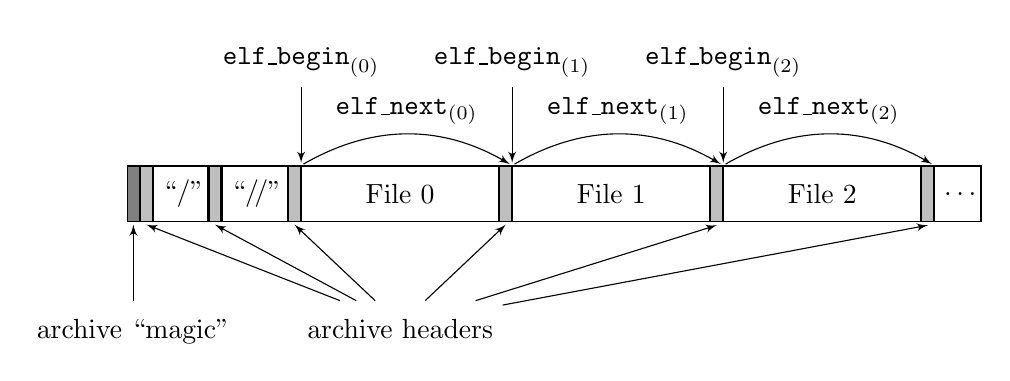
\begin{tikzpicture}[
    file/.style={               % Boxes denoting file content.
      rectangle,
      draw,
      text centered,
      text width=6.45em,
      node distance=0pt,
      minimum height=2em
    },
    header/.style={             % Boxes denoting archive headers.
      rectangle,
      draw,
      fill=black!25,
      node distance=0pt,
      minimum height=2em,
      minimum width=1ex,
      inner sep=0pt,
    },
    lbl/.style={                % Styling of label text.
      text height=1em
    }]

    % Depict the structure of the archive pictorially.
    \node[header,fill=black!50] (magic) {};
    \node[header] (s0) [right=of magic] {};
    \node[file,text width=1.3em] (symtab) [right=of s0] {``/''};
    \node[header] (s1) [right=of symtab] {};
    \node[file,text width=1.7em] (strtab) [right=of s1] {``$/\!/$''};
    \node[header] (h0) [right=of strtab] {};
    \node[file]   (f0) [right=of h0] {File 0};
    \node[header] (h1) [right=of f0] {};
    \node[file]   (f1) [right=of h1] {File 1};
    \node[header] (h2) [right=of f1] {};
    \node[file]   (f2) [right=of h2] {File 2};
    \node[header] (h3) [right=of f2] {};
    \node[file,text width=1em] (f3) [right=of h3] {$\ldots$};

    % Label the parts of the archive.
    \node[lbl] (lmagic) [below=of magic,text height=1em] {archive ``magic''}
      edge [->] ([yshift=-1pt] magic.south);
    \node[lbl] (lheader) [below=of f0.south,text height=1em] {archive headers}
      edge [->] ([yshift=-1pt] s0.south)
      edge [->] ([yshift=-1pt] s1.south)
      edge [->] ([yshift=-1pt] h0.south)
      edge [->] ([yshift=-1pt] h1.south)
      edge [->] ([yshift=-1.2pt] h2.south)
      edge [->] ([yshift=-1.2pt] h3.south);

    % Label the contents retrieved by calls to elf_begin().
    \node[lbl] (eb0) [above=of f0.north west] {$\texttt{elf\_begin}_{(0)}$}
      edge[->] ([yshift=1pt] f0.north west);
    \node[lbl] (eb1) [above=of f1.north west] {$\texttt{elf\_begin}_{(1)}$}
      edge [->] ([yshift=1pt] f1.north west);
    \node[lbl] (eb2) [above=of f2.north west] {$\texttt{elf\_begin}_{(2)}$}
      edge [->] ([yshift=1pt] f2.north west);

    % Show the traversal of the archive by elf_next().
    \draw[->,shorten >=1pt,shorten <=1pt,bend left] (h0.north east) to
      node[auto] {$\texttt{elf\_next}_{(0)}$} (h1.north east);
    \draw[->,shorten >=1pt,shorten <=1pt,bend left] (h1.north east) to
      node[auto] {$\texttt{elf\_next}_{(1)}$} (h2.north east);
    \draw[->,shorten >=1pt,shorten <=1pt,bend left] (h2.north east) to
      node[auto] {$\texttt{elf\_next}_{(2)}$} (h3.north east);
  \end{tikzpicture}
  \caption{Iterating through \tool{ar} archives with
    \function{elf\_begin} and \function{elf\_next}.}\label{fig.ariter}
\end{figure}

\begin{callout}{prog6}
  \lstinputlisting[caption=Program 6, label=src.prog.6]{prog6.txt}

  \begin{description}
  \item[\coref{1}] We open the archive for reading.
  \item[\coref{2}] We obtain an \type{Elf} descriptor by calling the
    function \function{elf\_begin}.\index{ar~archive!reading of}
    We then verify that the \library{libelf} library has recognized
    the file as an \tool{ar} archive.

  \item[\coref{3}] We call the \function{elf\_begin} to obtain a
    nested \type{Elf} descriptor to an archive member.  The third
    parameter passed to \function{elf\_begin} is a pointer to the
    \type{Elf} descriptor for the archive itself.

  \item[\coref{4}] We retrieve the archive header for the current
    archive member using the function \function{elf\_getarhdr}. This
    function will translate the file names in the archive header to
    \code{NUL}-terminated strings suitable for use with
    \code{printf}.\index{ar~archive!header!retrieval~of}

    Figure~\vref{fig.arhdr} shows the translated information returned
    by \function{elf\_getarhdr}.

    \begin{lstlisting}[caption=The \type{Elf\_Arhdr} Structure,
        label=fig.arhdr, basicstyle=\small\ttfamily]
typedef struct {
    time_t      ar_date;     /* time of creation */
    char        *ar_name;    /* archive member name */
    gid_t       ar_gid;      /* creator's group */
    mode_t      ar_mode;     /* file creation mode */
    char        *ar_rawname; /* 'raw' member name */
    size_t      ar_size;     /* member size in bytes */
    uid_t       ar_uid;      /* creator's user id */
} Elf_Arhdr;
    \end{lstlisting}

    We then print out the name and the size of the member using the
    \parameter{ar\_name} and \parameter{ar\_size} fields of the
    returned \type{Elf\_Arhdr} structure.

  \item[\coref{5}] We call the \function{elf\_next} function to set up
    the parent archive descriptor (held in the variable \code{ar}
    in our example) to return the next archive member on the next call
    to function \function{elf\_begin}.

    The \function{elf\_next} function will return the value
    \constant{ELF\_C\_READ} as long as the traversal of the archive
    can continue.  When called with a descriptor to the last member of
    an archive the \function{elf\_next} function will return the value
    \constant{ELF\_C\_NULL}.  This value will cause the subsequent
    call to function \function{elf\_begin} at step 3 to return
    \code{NULL}, thereby terminating the loop.

    Figure \vref{fig.ariter} shows how the functions
    \function{elf\_begin} and \function{elf\_next} work together to
    step through an \tool{ar} archive.%
    \index{ar~archive!sequential~access}

  \item[\coref{6}] We call \function{elf\_end} to release the
    resources held by \type{Elf} descriptors that are no longer
    needed.
  \end{description}
\end{callout}

Save the program in listing~\ref{src.prog.6} to a file named
\filename{prog6.c}, and compile and run it as shown.
\index{libelf@\texttt{libelf}!linking with}

\begin{callout}{scr6}
  \begin{lstlisting}[language={}, basicstyle=\small\ttfamily,
      label=scr.prog6, caption=Compiling and Running prog6]
% cc -o prog6 prog6.c -lelf @\co{1}@
% ./prog6 /usr/lib/librt.a @\co{2}@
             timer.o 7552
                mq.o 8980
               aio.o 8212
      sigev_thread.o 15528
  \end{lstlisting}
  \begin{description}
  \item[\coref{1}] We compile and link the program with \library{libelf}.
  \item[\coref{2}] We run the program on an archive and obtain a
    listing of the archive's contents.
  \end{description}
\end{callout}

\chapter{Conclusion}\label{chap.conclusion}

This tutorial covered the following topics:
\begin{itemize}
\item We gained an overview of the facilities offered by
  \library{libelf} for manipulating ELF objects.
\item We studied the basics of the ELF format. We looked at a few key
  ELF data structures, and at their layout inside ELF objects.
\item We wrote example programs that retrieved and displayed the ELF
  data structures present in a few ELF objects.
\item We looked at how to create new ELF objects using the
  \library{libelf} library.
\item We looked at how to read \tool{ar} archives using
  \library{libelf}.
\end{itemize}

\section{Further Reading}

\index{ELF!further reading}

\subsection{On the Web}
Peter Seebach's DeveloperWorks article ``\href{%
https://web.archive.org/web/20070224140341/http://www-128.ibm.com/developerworks/power/library/pa-spec12/%
}{An unsung hero: The hardworking ELF}'' covers the history and
features of the ELF format. Hongjiu Liu's ``\href{%
https://citeseerx.ist.psu.edu/viewdoc/summary?doi=10.1.1.37.8698}{ELF:
From The Programmer's Perspective}'' describes how to use the
features of ELF with GCC and GNU ld.  The paper ``\href{%
http://citeseerx.ist.psu.edu/viewdoc/summary?doi=10.1.1.136.2517}{Extending
Sim286 to the Intel386 Architecture with 32-bit processing and Elf
Binary input} by Michael L. Haungs and Brian A. Malloy contains a
description of the ELF format in the chapter ``\href{%
https://web.archive.org/web/20071217235525/www.cs.ucdavis.edu/~haungs/paper/node10.html%
}{Executable and Linking Format (ELF)}''.

Neelakanth Nadgir's tutorial ``\href{%
https://web.archive.org/web/20110926220119/http://developers.sun.com/solaris/articles/elf.html%
}{LibElf and GElf - A Library to Manipulate ELf Files}'' is a readable
introduction to the ELF(3) and GELF(3) APIs in Solaris\trade.

\index{linking!books about}The
\href{https://docs.oracle.com/cd/E53394_01/html/E54813/index.html}{Linkers
and Libraries Guide} from Oracle\reg describes the linking and
loading tools present in Solaris\trade.  Chapter 14 of this book,
titled ``Object File Format'', contains a readable introduction to the
ELF format.

\subsection{More Example Programs}

\index{libelf@\texttt{libelf}!additional examples}
The
\href{https://sourceforge.net/p/elftoolchain/code/HEAD/tree/trunk/}%
{source code for the tools} being developed at the
\elftoolchainproject at \href{https://sourceforge.net/}{SourceForge.Net}
show the use of the ELF(3)/GELF(3) APIs in useful programs.

For readers looking for smaller programs to study, Emmanuel Azencot
offers a website with
\href{http://freemanu1.free.fr/elf_examples/index.html}{example
  programs}.

\subsection{Books}

\index{linking!books about}John Levine's
``\href{https://linker.iecc.com/}{Linkers and Loaders}'' is a readable
book offering a overview of the process of linking and loading object
files.

\subsection{Standards}

\index{ELF!specification}The current specification of the ELF
format, the ``\href{https://refspecs.linuxbase.org/elf/elf.pdf}%
{Tool Interface Standard (TIS) Executable and Linking Format
(ELF) Specification, Version 1.2}'' is freely available to download.

\section{Getting Further Help}

\index{getting help!mailing list}If you have further questions about
the use of \library{libelf}, please feel free to use our discussion
list: \texttt{elftoolchain-\-developers@lists.sourceforge.net}.

\backmatter

% Typeset an index.
\printindex
\end{document}
